%%%%%%%%%%%%%%%%%%%%%%%%%%%%%%%%%%%%%%%%%%%%%%%%%%%%
\newcommand{\Ademi}{\Aa\pa{ \half }}

\newcommand{\bgaA}{\bga {\scriptscriptstyle \! \bullet \!} \bA}
\newcommand{\infga}{\underline{\ga}}
\newcommand{\supga}{\overline{\ga}}

\newcommand{\PS}{P_{\bSs}}
\newcommand{\PSp}{P_{\bSs^\bot}}
\newcommand{\RS}{R_{\bSs}}
\newcommand{\JgA}{J_{\bgaA}}
\newcommand{\RgA}{R_{\bgaA}}
\newcommand{\JgAi}{J_{\!\frac{\ga}{w_i}\!A_i}}
\newcommand{\RgAi}{R_{\!\frac{\ga}{w_i}\!A_i}}
\newcommand{\JgiAi}{J_{\!\ga_i\!A_i}}
\newcommand{\RgiAi}{R_{\!\ga_i\!A_i}}

\newcommand{\Tb}{\bT_{1,\bga}}
\newcommand{\Tf}{\bT_{2,\ga}}
\newcommand{\bBJ}{\bB\PS}
\newcommand{\Apga}{\bA_{\bga}\prim}
\newcommand{\Apgat}{\bA_{\bga_k}\prim}
\newcommand{\Apgainf}{\bA_{\bgainf}\prim}
\newcommand{\projS}{\PS}
\newcommand{\projP}{\PSp}
\newcommand{\pSs}[1]{{#1}^{\bSs}}
\newcommand{\pSp}[1]{{#1}^{\boldsymbol \bot}}
\newcommand{\Fx}{\mathbf{F}}

\newcommand{\musp}{\mu}
\newcommand{\mutv}{\nu}
\newcommand{\normbk}[1]{\norm{#1}_{1,2}^{\Bb}}
\newcommand{\normtv}[1]{\norm{#1}_{\mathrm{TV}}}
\newcommand{\normbki}[1]{\norm{#1}_{1,2}^{\Bb_i}}
\newcommand{\normbktv}[1]{\norm{#1}_{1,2}^{\Bb_{\mathrm{TV}}}}

\newcommand{\RNN}{\Ii}
\newcommand{\RNJ}{\Ii^J}
\newcommand{\RG}{\Ii^2}
\newcommand{\Ks}{K}
\newcommand{\Mr}{M}

\newcommand{\gradient}{\grad}

\newcommand{\GFB}{\textsc{GFB}\xspace}
\newcommand{\DR}{\textsc{DR}\xspace}
\newcommand{\ChPo}{\textsc{ChPo}\xspace}
\newcommand{\CoPe}{\textsc{CoPe}\xspace}
\newcommand{\HPE}{\textsc{HPE}\xspace}
%%%%%%%%%%%%%%%%%%%%%%%%%%%%%%%%%%%%%%%%%%%%%%%%%%%%

%%%%%%%%%%%%%%%%%%%%%%%%%%%%%%%%%%%%%%%%%%%%%%%%%%%%
%%%%%%%%%%%%%%%%%%%%%%%%%%%%%%%%%%%%%%%%%%%%%%%%%%%%
%%%%%%%%%%%%%%%%%%%%%%%%%%%%%%%%%%%%%%%%%%%%%%%%%%%%
\section{Introduction}

Throughout this paper, $\Hh$ denotes a real Hilbert space endowed with scalar product $\dprod{\cdot}{\cdot}$ and associated norm $\norm{\cdot}$, $\Id$ is the identity operator on $\Hh$, and $n$ is a positive integer.

%%%%%%%%%%%%%%%%%%%%%%%%%%%%%%%%%%%%%%%%%%%%%%%%%%%%
\subsection{Structured Monotone Inclusion and Minimization Problems}

We consider the following monotone inclusion problem
%
\begin{equation}\label{eq:incl}
	\sobjs{Find} x \in \left\{ \zer \pa{ B + \textsum{i=1}{n} A_i x } \eqdef \setdef{ x \in \Hh }{ 0 \in B x + \textsum{i=1}{n} A_i x } \right\}~,
\end{equation}
%
where $B : \Hh \mapsto \Hh$ is cocoercive, and for all $i$, $A_i : \Hh \mapsto 2^\Hh$ is a maximal monotone set-valued map.
While such inclusion problems arise in various fields, our main motivation is to solve convex minimization problems. Indeed, it is well-known that the subdifferential $\partial g_i$ of a function $g_i \in \Ga_0(\Hh)$ is a maximal monotone map; $\Ga_0(\Hh)$ being the class of lower semicontinuous, proper, convex function from $\Hh$ to $]\minfty,\pinfty]$. If moreover $f \in \Ga_0(\Hh)$ is differentiable with a Lipschitz continuous gradient, then Baillon-Haddad's theorem \cite{BaillonHaddad77} asserts that $\nabla f$ is cocoercive. Defining $F \eqdef f + \textsum{i=1}{n} g_i$, the set of minimizers of $F$ verifies
%
\[
	\argmin F = \zer \pa{ \nabla f + \textsum{i=1}{n} \partial g_i }~,
\]
%
provided that the following conditions hold
%
\begin{enumerate}[label={\rm (H\arabic{*})}, ref={\rm (H\arabic{*})}]
\item \label{H:argmin} $\argmin F \neq \emptyset$,
\item \label{H:sri} $(0,\ldots,0) \in \sri\{(x-y_1,\ldots,x-y_n) ~ \big | x \in \Hh \sobjs{and} \foralls i, \, y_i \in \dom g_i\}$,
\end{enumerate}
%
where $\dom g \eqdef \{x \in \Hh \big | g(x) < \pinfty\}$ denotes the domain of a function $g$ and $\sri C$ denotes the strong relative interior of a non-empty convex subset $C$ of $\Hh$ \cite{BauschkeCombettes11}. Therefore, identifying $B$ with $\nabla f$ and the $A_i$'s with the $\partial g_i$'s, solving \eqref{eq:incl} allows to solve
%
\begin{equation}\label{eq:min}
	\umin{x \in \Hh} \{ F(x) \eqdef f(x) + \textsum{i=1}{n} g_i(x) \}~.
\end{equation}
%

The structured monotone inclusion problem \eqref{eq:incl} is fairly general, and a wide range of iterative algorithms to solve it take advantage of the specific properties of the operators involved in the summand. As we will see, one crucial property is the possibility to compute the \textit{resolvent} of a maximal monotone operator $A$, denoted $J_A$. It is defined as (see Section~\ref{sec:defn-prop} for details)
%
\[ J_A x = y \quad \equivdef \quad x \in y + A y~. \]
%
For a given $x \in \Hh$, computing $J_A x$ is in itself a monotone inclusion problem, but it turns out that it can be solved explicitly for many operators, \eg the action of the resolvent can be easily computed in closed form. Our interest is in \textit{splitting} methods to solve \eqref{eq:incl}: iterative algorithms that evaluate individually the operator $B$ (cocoercive) and the resolvents $J_{A_i}$, at various points of $\Hh$, but not the resolvents of sums.
%The key point of a decomposition like \eqref{eq:incl} is that one may have access to the resolvent of each isolated $A_i$, but not to the resolvent of their sum; hence the term of \textit{splitting}. In this paper, we furthermore take advantage of the cocoercivity of one of the summand.

The next section recall several important previous works on splitting algorithms, focusing on their application to convex optimization.

%%%%%%%%%%%%%%%%%%%%%%%%%%%%%%%%%%%%%%%%%%%%%%%%%%%%
\subsection{Splitting Methods for Minimization Problems}

If $g$ is a function in $\Ga_0(\Hh)$, the resolvent of its subdifferential, $J_{\partial g}$, can be shown (see \sref{sec:defn-prop}) to be equal to the Moreau's proximity operator of $g$ \cite{Moreau65}, defined for all $x \in \Hh$ as
%
\[
	 \prox_{g}(x) \eqdef \uargmin{y \in \Hh} \, \half \norm{x - y}^2 + g(y)~.
\]
% 
Again, this can be solved explicitly for many functions; such functions are dubbed ``simple''.

Another important property of some part of a functional to be minimized is differentiability. Recalling \eqref{eq:min}, the forward-backward algorithm applies if $f$ is differentiable with a Lipschitz continuous gradient, and ${n \equiv 1}$ with $g_1$ simple. This scheme consists in performing alternatively a gradient-descent (corresponding to an explicit step on the function $f$) followed by a proximal step (corresponding to an implicit step on the function $g_1$). Such a scheme can be understood as a generalization of the projected gradient method. This algorithm, which finds its roots in numerical analysis for PDE's, has been well studied for solving monotone inclusion and convex optimization problems \cite{Bredies08,ChenRockafellar97,CombettesWajs05,Gabay83,Mercier79,Passty79,Tseng91,Tseng00}. Accelerated multistep versions or convex optimization have been proposed~\cite{BeckTeboulle09,Nesterov07,Tseng08}, that enjoy a faster convergence rate of $O(1/k^2)$ on the objective $F$ in the general case, where $k$ is the iteration counter.

Other splitting methods do not require any smoothness on any part of the composite functional $F$. The Douglas-Rachford scheme was originally developed to find the zeros of the sum of two linear operators \cite{DouglasRachford56}, and then two non-linear operators in \cite{Lieutaud69} or two maximal monotone operators in \cite{LionsMercier79}, see also \cite{Combettes04,EcksteinBertsekas92}. This scheme applies to minimizing $g_1 + g_2$, provided that $g_1$ and $g_2$ are simple. The backward-backward algorithm~\cite{AckerPrestel80,Bauschke05,Combettes04,Lions78,Passty79} can be used to minimize $F = g_1 + g_2$ when the functions involved are the indicator functions of non-empty closed convex sets, or involve Moreau envelopes.  Interestingly, if one of the functions $g_1$ or $g_2$ is a Moreau envelope and the other is simple, the backward-backward algorithm amounts to a forward-backward scheme.

If $L$ is a bounded injective linear operator, it is possible to minimize $F = g_1 \circ L + g_2$ by applying these splitting schemes on the Fenchel-Rockafellar dual problem. It was shown that applying the Douglas-Rachford scheme leads to the alternating direction method of multipliers (ADMM)~\cite{EcksteinBertsekas92,FortinGlowinski83,Gabay83,GabayMercier76,GlowinskiLeTallec89}. For non-necessarily injective $L$ and $g_2$ strongly convex with a Lipschitz continuous gradient, the forward-backward algorithm can be applied to the Fenchel-Rockafellar dual \cite{Combettes10,FadiliPeyre10}. Dealing with an arbitrary bounded linear operator $L$ can be achieved using primal-dual methods motivated by the classical Kuhn-Tucker theory. Starting from methods to solve saddle function problems such as the Arrow-Hurwicz  method \cite{ArrowHurwicz58} and its modification \cite{Popov80}, the extragradient method \cite{Korpelevich76}, this problem has received a lot of attention more recently \cite{Briceno-AriasCombettes11,ChambollePock11,ChenTeboulle94,MonteiroSvaiter10,Solodov04,Tseng97}.

It is also possible to extend the Douglas-Rachford algorithm to an arbitrary number $n > 2$ of simple functions. Inspired by the method of partial inverses \cite[Section~5]{Spingarn83}, most methods rely either explicitly or implicitly on introducing auxiliary variables and bringing back the original problem to the case $n \equiv 2$ in the product space $\Hh^{n}$. Doing so yields iterative schemes in which one performs independent parallel proximal steps on each of the simple functions and then computes the next iterate by essentially averaging the results. Variants have been proposed in \cite{CombettesPesquet08}, and in \cite{EcksteinSvaiter09} who describe a general projective framework that does not reduce the problem to the case $n \equiv 2$. These extensions however do not apply to the forward-backward scheme that can only handle $n \equiv 1$. It is at the heart of this paper to present such an extension. 

Recently proposed methods extend existing splitting schemes to handle the sum of any number of $n \geq 2$ composite functions of the form $g_i = h_i \circ L_i$, where the $h_i$'s are simple and the $L_i$'s are bounded linear operators. Let us denote $\adj{L_i}$ the adjoint operator of $L_i$. If $L_i$ satisfies $L_i  \adj{L_i} = \nu \Id$ for any $\nu > 0$ (it is a so-called \textit{tight frame}), $h_i \circ L_i$ is simple as soon as $h_i$ is simple and $\adj{L_i}$ is easy to compute \cite{Combettes07a}. This case thus reduces to the previously reviewed ones. If $L_i$ is not a tight frame but $\pa{\Id + \adj{L_i} L_i}$ or $\pa{\Id + L_i \adj{L_i}}$ is easily invertible, it is again possible to reduce the problem to the previous cases by introducing as many auxiliary variables as the number of $L_i$'s each belonging to the range of $L_i$. Note however that, if solved with the Douglas-Rachford algorithm on the product space, the auxiliary variables are also duplicated, which would increase significantly the dimensionality of the problem. Some dedicated parallel implementations were specifically designed for the case where $\pa{\sum_i \adj{L_i} L_i}$ or $\pa{\sum_i L_i \adj{L_i}}$ is (easily) invertible, see for instance \cite{Eckstein94,PesquetPustelnik11}. If the $L_i$'s satisfy none of the above properties, it is still possible to call on primal-dual methods, either by writing $F = \sum_{i=1}^n h_i \circ L_i = g \circ L$ with $L(x) = \pa{L_i(x)}_i$ and $g \bpa{\pa{x_i}_i} = \sum_i h_i(x_i)$, see for instance~\cite{Dupe11b}; or on the product space $F \bpa{\pa{x_i}_i} = \sum_i h_i \pa{ L_i x_i } + \iota_{\bSs} \bpa{\pa{x_i}_i}$ \cite{Briceno-AriasCombettes11}, where $\iota_{\bSs}$ is the indicator function of the closed convex set $\bSs$ defined in \sref{sec:prod-space}.

In spite of the wide range of already existing proximal splitting methods, none seems satisfying to address explicitly the case where $n > 1$ and $f$ is smooth but not necessarily simple. A workaround that has been proposed previously used nested algorithms to compute the proximity operator of $\sum_i g_i$ within sub-iterations, see for instance~\cite{Chaux09,Dupe09}; this leads to practical as well as theoretical difficulties to select the number of sub-iterations. More recently, \cite{MonteiroSvaiter10} proposed an algorithm for minimizing $F = f + g$ under linear constraints. We show in \sref{sec:relations} how this can be adapted to address the general problem \eqref{eq:min} while achieving full splitting of the proximity operators of the $g_i$'s and using the gradient of $f$. In preparing a first draft of this manuscript, we became aware that other authors \cite{CombettesPesquet11,Condat11,Vu11} have independently and concurrently developed primal-dual algorithms to solve problems that encompass the one we consider here. These approaches and algorithms are however different from ours in many important ways. This will be discussed in detail in \sref{sec:relations} especially in relation to \cite{CombettesPesquet11}. We also report a suite of numerical experiments in \sref{sec:numeric} which suggest that our primal algorithm is more adapted for imaging problems of the form \eqref{eq:min}.

%%%%%%%%%%%%%%%%%%%%%%%%%%%%%%%%%%%%%%%%%%%%%%%%%%%%
\subsection{Applications in Image Processing}

Many imaging applications require solving ill-posed inverse problems to recover high quality images from low-dimensional and noisy observations. These challenging problems necessitate the use of regularization through prior models to capture the geometry of natural signals, images or videos. Numerical solution of inverse problems can be achieved through minimization of objective functionals, with respect to a high-dimensional variable, that takes into account both a fidelity term to the observations and regularization terms reflecting the priors. Clearly, such functionals are composite by construction, hence fitting in the framework of \eqref{eq:min}. \sref{sec:numeric} details several examples of such inverse problems.  

In many situations, this leads to the optimization of a convex functional that can be split into the sum of convex smooth and nonsmooth terms. The smooth part of the objective is in some cases a data fidelity term and reflects some specific knowledge about the forward model, \ie the noise and the measurement/degradation operator. This is for instance the case if the operator is linear and the noise is additive Gaussian, in which case the data fidelity is a quadratic function. The most successful regularizations that have been advocated are nonsmooth, which typically allow to preserve sharp and intricate structures in the recovered data. Among such priors, sparsity-promoting ones have become popular, \eg the $\ell_1$-norm of coefficients in a wisely chosen dictionary \cite{Mallat99}, or total variation (TV) prior~\cite{ROF92}. To better model the data, composite priors can be constructed by summing several suitable regularizations, see for instance the morphological diversity framework~\cite{FadiliStarckBook09}. The proximity operator of the $\ell_1$-norm penalization is a simple soft-thresholding~\cite{Donoho95}, whereas the use of complex or mixed regularization priors justifies the splitting of nonsmooth terms in several simpler functions (see \sref{sec:numeric} for concrete examples).

The composite structure of convex optimization problems raising when solving inverse problems in the form of a sum of simple and/or smooth functions involving linear operators explains the popularity of proximal splitting schemes in imaging science. Depending on the structure of the objective functional as detailed in the previous section, one can resort to the appropriate splitting algorithm. For instance, the forward-backward algorithm and its modifications has become popular for sparse regularization with a smooth data fidelity, see for instance~\cite{BeckTeboulle09,Briceno-Arias09,Chaux07,CombettesWajs05,Daubechies04,Fadili06,FigueiredoNowak03}. The Douglas-Rachford and its parallelized extensions were also used in a variety of inverse problems implying only nonsmooth functions, see for instance \cite{Briceno-Arias10,Chaux09,Combettes07a,CombettesPesquet08,Dupe11a,Dupe09,Dupe12,Pustelnik11}. The ADMM (which is nothing but Douglas-Rachford on the dual) was also applied to some linear inverse problems in \cite{Figueiredo10a,Figueiredo10b}. Primal-dual schemes \cite{ChambollePock11,Dupe11b} are among the most flexible schemes to handle more complicated priors. The interested reader may refer to \cite[Chapter 7]{FadiliStarckBook09} and \cite{CombettesPesquet09} for extensive reviews.

%%%%%%%%%%%%%%%%%%%%%%%%%%%%%%%%%%%%%%%%%%%%%%%%%%%%
\subsection{Contributions and Paper Organization}

This paper introduces a novel generalized forward-backward (\GFB) algorithm to solve the monotone inclusion \eqref{eq:incl}. The algorithm achieves full splitting where all operators are used separately: an explicit step for $B$ (single-valued) and a parallelized implicit step through the resolvent of the $A_i$'s. We prove convergence of the algorithm even when summable errors may contaminate the iterations. To the best of our knowledge, it is among the first algorithms to tackle the case where $n > 1$ (see \sref{sec:relations} for relation to other works). Although our numerical results are reported only on imaging applications, the algorithm may prove useful for many other applications such as machine learning, statistical estimation or optimal control.

\sref{sec:gfb} presents the algorithm and states our main theoretical result, before commenting on some relevant aspects and on alternatives in the literature. Numerical examples are reported in \sref{sec:numeric} to show the usefulness of this approach for imaging problems. The convergence proof is deferred to \sref{sec:proofs}, after recalling some preliminary results on monotone operator theory.

%%%%%%%%%%%%%%%%%%%%%%%%%%%%%%%%%%%%%%%%%%%%%%%%%%%%
%%%%%%%%%%%%%%%%%%%%%%%%%%%%%%%%%%%%%%%%%%%%%%%%%%%%
%%%%%%%%%%%%%%%%%%%%%%%%%%%%%%%%%%%%%%%%%%%%%%%%%%%%
\section{Generalized Forward-Backward Splitting}
\label{sec:gfb}

%%%%%%%%%%%%%%%%%%%%%%%%%%%%%%%%%%%%%%%%%%%%%%%%%%%%
\subsection{The Algorithmic Scheme}
\label{sec:algo}

We consider problem \eqref{eq:incl} where all operators are maximal monotone, $B$ is $\be$-cocoercive with $\be \in \, ]0,\pinfty[$, \ie
%
\begin{equation*}\label{eq:coco}
	\foralls x,y \in \Hh, \quad \be \norm{Bx - By}^2 \leq \dprod{Bx - By}{x - y}~,
\end{equation*}
% 
and for all $i$ and all $\ga > 0$, $J_{\!\ga\!A_i}$ (the resolvent of $\ga A_i$) is easy to compute. Our proposed generalized forward-backward algorithm is detailed in \aref{algo:gfb}. 

\begin{algorithm}[h]
\caption{A Generalized Forward-Backward Algorithm for solving \eqref{eq:incl}.\newline
$\be \in \, ]0,\pinfty[$ is a cocoercivity constant of $B$.}
{\noindent{\bf{Require}}}
 $\begin{array}{ll}
 {\pa{z_i}_{i \in \bbket{1,n}} \in \, \Hh^n}, & {\pa{w_i}_{i \in \, \bbket{1,n}} \in {]0,1]}^n \sobjs{s.t.} \sum_{i=1}^n w_i = 1}, \\
							    \ga \in \, ]0,2\be[, & \la_k \in \left] 0,\min\bpa{\frac{3}{2},\textfrac{1}{2}+\textfrac{\be}{\ga}} \right[ ~ \forall k \in \N ~. \end{array}$\\
{\noindent{\bf{Initialization}}}\\
$x \leftarrow \sum_i w_i z_i$;\\
$k \leftarrow 0$.\\
{\noindent{\bf{Main iteration}}}\\
\Repeat{convergence}{
	\For{$i \in \bbket{1,n}$}{
		\abovedisplayskip=0pt
		\belowdisplayskip=0pt
		\begin{flalign}\label{eq:core-gfb}
			z_i \leftarrow z_i + \la_k \bpa{ \JgAi \bpa{ 2x - z_i - \ga B x } - x}~;& &
		\end{flalign}
	}
	$x \leftarrow \sum_i w_i z_i$;\\
	$k \leftarrow k+1$.
}
{\noindent{\bf{Return}}} $x$.
\label{algo:gfb}
\end{algorithm}

To state our main theorem that ensures the convergence of the algorithm and its robustness to summable errors, for each $i$ let $\Eps_{1,k,i}$ be the error at iteration $k$ when computing $\JgAi$, and let $\Eps_{2,k}$ be the error at iteration $k$ when computing $B$. An inexact \GFB algorithm generates sequences $\pa{z_{i,k}}_{k \in \N}$, $i \in \bbket{1,n}$ and $\pa{x_k}_{k \in \N}$, such that for all $i \in \bbket{1,n}$ and $k \in \N$,
%
\begin{equation}\label{eq:gfb-err-algo}
	z_{i,k+1} = z_{i,k} + \la_k \bpa{ \JgAi \bpa{ 2 x_k - z_{i,k} - 
	\ga_k \pa{ B x_k + \Eps_{2,k} } } + \Eps_{1,k,i} - x_k } ~.
\end{equation}

\begin{theorem}
Suppose that $\zer \pa{ B + \textsum{i=1}{n} A_i } \neq \emptyset$. Suppose that the following assumptions are satisfied:
%
\begin{enumerate}[label={\rm (\roman{*})}, ref={\rm (\roman{*})}]
	\item{\label{h:lim-la-algo}} $0 < \inf_{k \in \N} \la_k \leq \sup_{k \in \N} \la_k < \min\bpa{\textfrac{3}{2},\textfrac{1}{2}+\textfrac{\be}{\ga}}$, and 
	\item{\label{h:sum-err-algo}} $\sum_{k=0}^{\pinfty} \norm{\Eps_{2,k}} < \pinfty$, and for all $i$, $\sum_{k=0}^{\pinfty} \norm{\Eps_{1,k,i}} < \pinfty$.
\end{enumerate}
%
Then the sequence $\pa{x_k}_{k \in \N}$ defined in \eqref{eq:gfb-err-algo} converges weakly towards a solution of \eqref{eq:incl}. Moreover, if $\foralls k \in \N, \, \la_k \leq 1$, then the convergence is strong if either $B$ is uniformly monotone, or $\bigtimes_{i=1}^n w_i^{-1} A_i$ is uniformly monotone. The latter is true for instance if $\forall i \in \bbket{1,n}$, $A_i$ is uniformly monotone with its modulus $\phy$ being also subadditive or convex.
\label{thm:gfb-algo}
\end{theorem}

\medskip

The definition of uniform monotonicity and the function $\phy$ is provided in Section~\ref{sec:defn-prop}.\\


The following corollary specializes \tref{algo:gfb} to the case of convex optimization problems of the form \eqref{eq:min}.
\begin{corollary}\label{cor:min}
Suppose that $\nabla f$ is Lipschitz continuous with constant $1/\be$, and that \ref{H:argmin}-\ref{H:sri} are verified. Substitute, in \aref{algo:gfb} and in \eqref{eq:gfb-err-algo}, $B$ with $\nabla f$ and $A_i$ with $\partial g_i$ (\ie $\JgAi$ with $\prox_{\!\frac{\ga}{w_i}\!g_i}$). Then under assumptions \ref{h:lim-la-algo}-\ref{h:sum-err-algo} of \tref{thm:gfb-algo}, the sequence $\pa{x_k}_{k \in \N}$ converges weakly towards a minimizer of \eqref{eq:min}. Moreover, if $\foralls k \in \N, \, \la_k \leq 1$, then $\pa{x_k}_{k \in \N}$ converges strongly to the unique minimizer of \eqref{eq:min} if either $f$ is uniformly convex, or $\bigtimes_{i=1}^n w_i^{-1} \partial g_i$ is uniformly monotone. The latter is true for instance if $\forall i \in \bbket{1,n}$, $g_i$ is uniformly convex with its modulus $\phy$ being also  subadditive or convex.
\end{corollary}

\medskip

The proofs are detailed in \sref{sec:proofs}. 
{~}\\

\begin{remark}
Recall that a function $f \in \Ga_0(\Hh)$ is uniformly convex of modulus $\phy: [0,\pinfty[ \to [0,\pinfty]$ if $\phy$ is a non-decreasing function that vanishes only at 0, such that for all $x$ and $y$ in $\dom f$, the following holds
%
\begin{equation*}
\foralls \rho \in ]0,1[, \, f(\rho x + (1-\rho) y) + \rho(1-\rho)\phy(\norm{x-y}) \leq \rho f(x) + (1-\rho)f(y)~.
\end{equation*}
%
\end{remark} 

\medskip

The formulation of \aref{algo:gfb} is general, but it can be simplified for practical purposes. In particular, the auxiliary variables $z_i$ can all be initialized to $0$, the weights $w_i$ set equally to $1/n$, and for simplicity the relaxation parameters $\lambda_k$ can be set to $1$, constant along iterations. This is what has been done in the numerical experiments described in \sref{sec:numeric}. 

%%%%%%%%%%%%%%%%%%%%%%%%%%%%%%%%%%%%%%%%%%%%%%%%%%%%
\subsection{Special instances}
\label{sec:hybrid}

Our \GFB algorithm can be viewed as a hybrid splitting algorithm whose special instances turn out to be classical splitting methods; namely the forward-backward and Douglas-Rachford algorithms.

\paragraph{Relaxed Forward-Backward}
For $n \equiv 1$, the core update operator \eqref{eq:core-gfb} of \aref{algo:gfb} specializes to
%
\begin{equation*}
	x \leftarrow x + \la_k \pa{ J_{\ga A} \pa{ x - \ga B x } - x }~,
\end{equation*}
%
so that $x_k$ given by \eqref{eq:gfb-err-algo} follows the iterations of the relaxed forward-backward algorithm \cite[Section~6]{Combettes04}. In this case, convergence can be ensured with step-size $\ga$ varying along iterations, see discussion in \rref{rem:nonstat}. For convex minimization problems, known results on convergence rate analysis (on the objective in general) and accelerated versions of the forward-backward algorithm \cite{BeckTeboulle09,Bredies08,Nesterov07,Tseng08} might be inspiring to study those of our \GFB (for the case where $\beta > 0$).

\paragraph{Relaxed Douglas-Rachford}
If we set $B \equiv 0$, the update of the auxiliary variables in \eqref{eq:core-gfb} becomes
%
%
\begin{equation*}
z_i \leftarrow z_i + \la_k \bpa{ \JgAi \bpa{ 2x - z_i } - x}~,
\end{equation*}
% 
so that $\pa{z_{i,k}}_i$ given by \eqref{eq:gfb-err-algo} follow the iterations of the relaxed Douglas-Rachford algorithm on the product space $\Hh^n$ for solving $0 \in \sum_i A_i x$ \cite{CombettesPesquet08,Spingarn83}. The convergence statements of \tref{thm:gfb}-\ref{claim:Tz}-\ref{claim:x} hold by replacing the conditions on the relaxation parameters by $\foralls k \in \NN, \, \la_k \in ]0,2[$ and $\sum_{k \in \N} \la_k(2-\la_k) = \pinfty$; this extends \rref{rem:ext-la} to $\al = \half$, by \pref{prop:Tb} (see \sref{sec:convergence}).

\paragraph{Resolvents of the sum of monotone operators}
Our \GFB scheme provides yet another way for computing the resolvent of the sum of maximal monotone operators $\pa{A_i}_i$. Given a point $y \in \ran \pa{\Id + \sum_i A_i}$, set in \eqref{eq:incl} $B: x \mapsto x - y$ and $\be \equiv 1$. It would be interesting to compare this algorithm with the Douglas-Rachford and Dykstra-based variants \cite{Combettes09b}. This is left to a future work.

\subsection{Relation to other works}
\label{sec:relations}

\paragraph{Relation to \cite{MonteiroSvaiter10}}
The authors in \cite[Section 5.3, (51)]{MonteiroSvaiter10} describe an instance of the ``block-decomposition'' hybrid proximal extragradient (HPE) for minimizing $F = f+g$ under linear constraints. \eqref{eq:min} can be cast in an equivalent linearly constraint convex programming
%
\begin{equation}\label{eq:HPE}
	\umin{\bz = \pa{z_i}_i \in \Hh^n} ~ f\pa{ \scriptstyle{\sum_i} \displaystyle w_i z_i } + \sum_i g_i(z_i) \qobjq{such that} \PSp(\bz) = \mathbf{0}~,
\end{equation}
% 
where $\PSp$ is the orthogonal projector on the subspace $\bSs^\bot \eqdef \setdef{\bz = \pa{z_i}_i \in \Hh^n}{\sum_i w_i z_i = 0}$. As $\PSp$ is self-adjoint, $\bz$ is an optimal solution if and only if there exists $\bv=\pa{v_i}_i \in \Hh^n$ such that 
\[
\mathbf{0} \in \bpa{ \nabla f \pa{ \scriptstyle{\sum_j} \displaystyle w_j z_j} }_i + \pa{ \partial g_i(z_i)/w_i }_i + \PSp(\bv) \qobjq{and} \PSp(\bz) = 0 ~,
\]
and the minimizer of $F$ is given by $x = \sum_i w_i z_i$.

Let $\syg \in ]0,1]$ and $\ga = \syg \frac{2 \syg \be}{1+\sqrt{1+4\syg^2\be^2}}$. Transposed to our setting, their iterations are presented in \aref{algo:HPE}.

\begin{algorithm}[h]
\caption{Iterations of Block-Decomposition HPE \cite{MonteiroSvaiter10}.}
\Repeat{convergence}{
\For{$i \in \bbket{1,n}$}{%
		 $\displaystyle z_i \leftarrow \prox_{\frac{\ga}{w_i} g_i} \bpa{ \ga^2 x + \pa{ 1 - \ga^2 } z_i - \ga \nabla f(x) + \ga \pa{v_i - u} }$;%
	}
\For{$i \in \bbket{1,n}$}{%
		 $\displaystyle v_i \leftarrow v_i - \ga z_i + \ga x$;%
	}
$x \leftarrow \sum_i w_i z_i$;\\
$u \leftarrow \sum_i w_i v_i$.
}
\label{algo:HPE}
\end{algorithm}

\noindent The update of the $z_i$'s in this iteration bears similarities with the one in \aref{algo:gfb}, where the $\ga$'s play analogous roles. Nonetheless, the two algorithms are different. For instance, our algorithm solves the primal problem while theirs solves both the primal and dual problems. In addition, the objective in \cite{MonteiroSvaiter10} is to study complexity, hence the different set of assumptions.

In preparing a revised draft of this manuscript, it came to our attention that an other adaptation of the block-decomposition HPE, exploiting the specific properties of the linear constraints $\PSp(\bz) = 0$ and changing the metric, leads to the iterations \eqref{eq:gfb-err-algo} with $\foralls k \in \N, \, \la_k = 1$, \ie no under- nor over-relaxation. This could be an other framework to study convergence properties of \GFB.
 
\paragraph{Relation to \cite{CombettesPesquet11}}
These authors independently developed another algorithm to solve a general class of problems that covers \eqref{eq:incl}. They rely on the classical Kuhn-Tucker theory and propose a primal-dual splitting algorithm for solving monotone inclusions involving a mixture of sums, linear compositions, and parallel sums (inf-convolution in convex optimization) of set-valued and Lipschitz operators. More precisely, the authors exploit the fact that the primal and dual problems have a similar structure, cast the problem as finding a zero of the sum of a Lipschitz continuous monotone map with a maximal monotone operator whose resolvent is easily computable. They solve the corresponding monotone inclusion using an inexact version of Tseng's forward-backward-forward splitting algorithm \cite{Tseng00}.

Removing the parallel sum, taking the linear operators as the identity in \cite[(1.1)]{CombettesPesquet11}, and assuming that the Lipschitz part is also cocoercive, one recovers problem \eqref{eq:incl}. For the sake of simplicity and space saving we do not reproduce here in full their algorithm. However, adapted to the optimization problem $\min_{x\in\Hh} f(x)+\sum_i g_i(L_ix)$, where each $L_i$ is a bounded linear operator, their scheme is presented in \aref{algo:CoPe} ($\adj{g_i}$ is the \textit{Legendre-Fenchel conjugate} of $g_i$).

\begin{algorithm}[h]
\caption{Iterations of Primal-Dual Algorithm of \cite{CombettesPesquet11}.
\label{algo:CoPe}}
Choose a sequence $\pa{\ga_k}_{k \in \N}$ in $[\epsilon,(1-\epsilon)/\zeta]$, where $\zeta \eqdef \beta^{-1} + \sqrt{\sum_i \norm{L_i}^2}$ and $\epsilon \in ]0,1/(1+\zeta)[$.\\
$k \leftarrow 0$.\\
\Repeat{convergence}{
$y \leftarrow x - \ga_k \pa{\nabla f(x) + \sum_{i=1}^n \adj{L_i}\pa{v_i}}$\\
\For{$i \in \bbket{1,n}$}{
	$\displaystyle z_i \leftarrow v_i + \ga_k L_i\pa{x}$;\\
	$\displaystyle v_i \leftarrow v_i - z_i + \prox_{\ga_k \adj{g_i}}(z_i) + \ga_k L_i\pa{y}$;
	}
$x \leftarrow x - \ga_k \pa{ \nabla f \pa{y} + \sum_{i=1}^n \adj{L_i} \bpa{ \prox_{\ga_k \adj{g_i}}(z_i) } }$;\\
$k \leftarrow k+1$
}
\end{algorithm}

\noindent Recall that the proximity operator of $\adj{g_i}$ can be easily deduced from that of $g_i$ using Moreau's identity. Taking $L_i=\Id$ in \aref{algo:CoPe} solves \eqref{eq:min}. While we solve the primal problem, their algorithm solves both the primal and dual ones. Note however that it requires two calls to the gradient of $f$ per iteration.

%%%%%%%%%%%%%%%%%%%%%%%%%%%%%%%%%%%%%%%%%%%%%%%%%%%%
%%%%%%%%%%%%%%%%%%%%%%%%%%%%%%%%%%%%%%%%%%%%%%%%%%%%
%%%%%%%%%%%%%%%%%%%%%%%%%%%%%%%%%%%%%%%%%%%%%%%%%%%%
\section{Numerical experiments}
\label{sec:numeric}

This section exemplifies the applicability of our \GFB splitting algorithm on image processing problems by solving some regularized inverse problems. The problems are selected so that other splitting algorithms can be applied as well and compared fairly. The parameters involved were manually selected for each compared algorithm to achieve its best performance, for instance in terms of energy decay. In the following, $\Id$ denotes the identity operator on the appropriate space to be understood from the context, $N$ is a positive integer and $\RNN \equiv \R^{N \times N}$ is the set of images of size $N \times N$ pixels.

%%%%%%%%%%%%%%%%%%%%%%%%%%%%%%%%%%%%%%%%%%%%%%%%%%%%
\subsection{Variational Image Restoration}

We consider a class of inverse problem regularizations, where one wants to recover an (unknown) high resolution image $y_0 \in \RNN$ from noisy low resolution observations $y = \Phi y_0 + w \in \RNN$. We report results using several ill-posed linear operators $\Phi : \RNN \to \RNN$, and focus our attention on convolution and masking operator, and a combination of these operators. In the numerical experiments, the noise vector $w \in \RNN$ is a realization of an additive white Gaussian noise of variance $\sig_w^2$.

The restored image $\widehat{y}_0=W\widehat{x}$ is obtained by optimizing the coefficients $\widehat{x} \in \Hh$ in a redundant wavelet frame~\cite{Mallat99}, where $W : \Hh \to \RNN$ is the wavelet synthesis operator. The wavelet atoms are normalized so that $W$ is a Parseval tight frame, \ie it satisfies $W\adj{W} = \Id$. In this setting, the coefficients are vectors $x \in \Hh\equiv \RNJ$ where the redundancy $J=3 J_0 + 1$ depends on the number of resolutions levels $J_0$ of the wavelet transform.

The general variational problem for the recovery reads
%
\begin{equation}\label{eq:vpb}
  \umin{x \in \Hh} \{F(x) \equiv \half \norm{y - \Phi W x}^2 + \musp \normbk{x} + \mutv \normtv{W x}\} ~.
\end{equation}
%
The first term in the summand is the \textit{data-fidelity} term, which is taken to be a squared $\ell_2$-norm to reflect the additive white Gaussianity of the noise. The second and third terms are \textit{regularizations}, enforcing priors assumed to be satisfied by the original image. The first regularization is a $\ell_1/\ell_2$-\textit{norm by blocks}, inducing structured sparsity on the solution. The second regularization is a discrete \textit{total variation semi-norm}, inducing sparsity on the gradient of the restored image. The scalars $\musp$ and $\mutv$ are weights -- so-called regularization parameters -- to balance between each terms of the energy $F$. We now detail the properties of each of these three terms.

	\subsubsection{Data-Fidelity $\half \norm{y - \Phi W x}^2$}
	\label{sec:data-fid}

For the inpainting inverse problem, one considers a masking operator 
%
\begin{equation*}
  \pa{\Mr \, y}_p \eqdef \begin{cases}
	0    & \sobjs{if} p \in \Om~, \\
        y_p  & \sobjs{otherwise~,}   \end{cases}
\end{equation*}
%
where $\Om$ is a set of pixels, taking into account missing or defective sensors; we will denote $\rho = \abs{\Om}/N^2$ the ratio of missing pixels. For the deblurring inverse problem, we consider a convolution with a discrete Gaussian filter of width $\sig_{\Ks}$, $\Ks : y \mapsto G_{\sig_{\Ks}} \ast y$, normalized to a unit mass. In the following, $\Phi$ will be either $\Mr$, $\Ks$ or the composition of both $\Mr  \Ks$.

\medskip

Denoting $L \eqdef \Phi W$, the fidelity term thus reads $f(x) = \half \norm{y - L x}^2$. The function $f$ corresponds to the smooth term in \eqref{eq:min}. Its gra\-dient $\nabla f : x \mapsto \adj{L} \pa{Lx - y}$ is Lipschitz continuous with constant $\beta^{-1} \leq \norm{\Phi W}^2 = 1$.

For any $\ga > 0$, the proximity operator of $f$ reads 
%
\begin{equation}\label{eq:prox-f}
 \prox_{\ga f}(x) = \inv{\pa{\Id+\ga \adj{L}L}}\pa{x+\ga \adj{L}y}.
\end{equation}
% 
The vector $\adj{L}y$ can be precomputed, but inverting $\Id+\ga \adj{L}L$ may be in general computationally demanding. For inpainting or deblurring alone, as $W$ is associated to a Parseval tight frame, the Sherman-Morrison-Woodbury formula gives
%
\begin{align}
  \inv{\pa{\Id+\ga \adj{L}L}} = & \Id - \adj{L} \inv{\pa{\Id+\ga L\adj{L}}} L \nonumber \\
			      = & \Id - \adj{W} \adj{\Phi} \inv{\pa{\Id+\ga \Phi \adj{\Phi} }} \Phi W \label{eq:prox-phi-w}~.
\end{align}
% 
Since $\Mr$ (resp. $\Ks$) is a diagonal operator in the pixel domain (resp. Fourier domain), \eqref{eq:prox-phi-w} can be computed in $O(N^2)$ (resp. $O(N^2 \log N)$) operations. However, the composite case $L \equiv \Mr \Ks W$ is more involved. A possible workaround\footnote{In this special case where $\Phi=\Mr \Ks$, an alternative would be to reapply the inversion lemma to \eqref{eq:prox-phi-w}. But this does not work in general unlike the auxiliary variables approach.} is to introduce an auxiliary variable, replacing $f : \Hh \to \R$ by ${\tilde{f} : \Hh \times \RNN \to ]\minfty,\pinfty]}$ defined by
%
\begin{equation}\label{eq:tilde-f}
  \tilde{f}(x,u) = \half \norm{y - \Mr u}^2 + \iota_{C_{\Ks W}}(x,u) = g_1(u) + g_2(x,u) ~,
\end{equation}
% 
where $C_{\Ks W} \eqdef \setdef{\pa{x,u} \in \Hh \times \RNN}{u = \Ks W x}$, and $\iota_C$ is the indicator function of the closed convex set $C$, i.e. $\iota_C(v)=0$ if $v \in C$, and $+\infty$ otherwise. Only then, $\prox_{\ga g_1}$ can be computed from \eqref{eq:prox-f}, and $\prox_{\ga g_2}$ is the orthogonal projection on ${\ker([\Id, -\Ks W])}$ \cite{Briceno-Arias10,Dupe11b}, which involves a similar inversion as in \eqref{eq:prox-phi-w}.

	\subsubsection{Regularization $\musp \normbk{x}$}
	\label{sec:spars-reg}

Sparsity-promoting regularizations with a syn\-thesis-type prior over wavelet (or other transformed) coefficients are popular to solve a wide range of inverse problems~\cite{Mallat99}. \cff{subfig:noblock} shows an example of orthogonal wavelet coefficients of a natural image where most of the coefficients have small amplitude. A way to enforce this ``sparsity'' is to include in \eqref{eq:vpb} the $\ell_1$-norm of the coefficients $\norm{x}_1 = \sum_p |x_p|$. 

The presence of edges or textures creates structured local dependencies in the wavelet coefficients of natural images. A way to take into account those dependencies is to replace the absolute value of the coefficients in the $\ell_1$-norm by the $\ell_2$-norm of groups (or \textit{blocks}) of coefficients \cite{PeyreFadili11,YuanLin06,Kowalski09,Chaux05,Elhamifar09}. This is known as the mixed $\ell_1/\ell_2$-norm, defined here as
%
\begin{equation}\label{eq:normbk}
  \normbk{x} = \sum_{\bk \in \Bb} \mu_\bk \norm{x_\bk} = \sum_{\bk \in \Bb} \mu_\bk \sqrt{\sum_{p \in \bk} x_p^2} ~,
\end{equation}
% 
where $p$ indexes the coefficients, the blocks $\bk$ are sets of indices, the \textit{block-structure} $\Bb$ is a collection of blocks and $x_\bk \eqdef \pa{x_p}_{p \in \bk}$ is a subvector of $x$ indexed by $\bk$. The positive scalars $\mu_\bk$ are weights tuning the influence of each block. \eqref{eq:normbk} defines a norm on $\Hh$ as soon as $\Bb$ covers the whole space, \ie $\foralls p \in \bbket{1,N}^2 \times \bbket{1,J}, \, \existss \bk \in \Bb : p \in \bk \sobjs{and} \mu_\bk > 0$. Note that for $\Bb \equiv \bigcup_p \cur{p}$ and $\mu_{ \cur{p} } \equiv 1$ for all $p$, it reduces to the $\ell_1$-norm.

We mentioned in the introduction that the proximal operator of the $\ell_1$-norm is the coefficient-wise soft-thresholding. Similarly, it is easy to show that whenever $\Bb$ is a disjoint partition where the blocks are \textit{non-overlapping}, \ie ${\foralls \bk,\bk\prim \in \Bb}, \, {\bk \cap \bk\prim = \emptyset}$, the proximity operator of $\normbk{\cdot}$ is the block-wise soft-thresholding
%
\begin{equation*}
  \prox_{\mu \normbk{\cdot}}\bpa{\pa{x_\bk}_\bk} = \bpa{\Th_{\mu_\bk \cdot \mu}(x_\bk)}_\bk ~,
\end{equation*}
%
with
%
\begin{equation*}
\Th_{\tau}(x_\bk) = 
\begin{cases}
0                                       & \sobjs{if} \norm{x_\bk} < \tau~, \\ 
\pa{ 1-\frac{\tau}{\norm{x_\bk}} } x_\bk & \sobjs{otherwise~,}
\end{cases}
\end{equation*}
%
and the coefficients $x_p$ not covered by $\Bb$ are left unaltered.

Non-overlapping block structures break the \textit{translation invariance} that is underlying most traditional image models. To restore this invariance, one can consider overlapping blocks, as illustrated in \cff{subfig:blocks2}. Computing $\prox_{\normbk{\cdot}}$ in this case is not as simple as for the non-overlapping case, because the blocks cannot be treated independently. For tree-structured blocks (\ie $\bk \cap \bk\prim \neq \emptyset \Rightarrow \bk \subset \bk\prim \sobjs{or} \bk\prim \subset \bk$), \cite{Jenatton10} proposes a method involving the computation of a min-cost flow. This could be computationally expensive and do not address the general case anyway. Instead, it is always possible to decompose the block structure as a finite union of non-overlapping sub-structures $\Bb = \bigcup_{i} \Bb_i$. The resulting term can finally be split into $\normbk{x} = \sum_{\bk \in \Bb} \norm{x_\bk} = \sum_i \sum_{\bk \in \Bb_i} \norm{x_\bk} = \sum_i \normbki{x}$, where each $\normbki{\cdot}$ is simple.

\begin{figure}[!ht]
\bigcenter
\subfigure[$\norm{x}_1 = \sum_p \abs{x_p}$]{
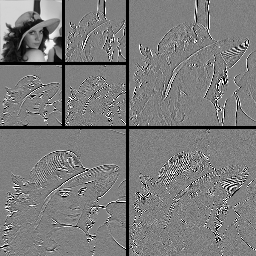
\includegraphics[width=4cm]{images/LaBouteWvlt.png}
\label{subfig:noblock}}
\subfigure[$\normbk{x} = \sum_{\color{red} \bk \in \Bb} \norm{x_{\color{red} \bk}}$]{
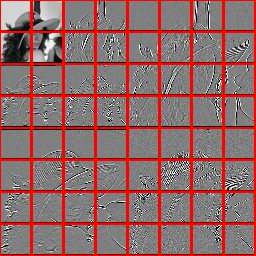
\includegraphics[width=4cm]{images/LaBouteWvltBlocks1.png}
\label{subfig:blocks1}}
\subfigure[$\normbk{x}%
= \norm{x}_{1,2}^{\textcolor{red}{\Bb_1}} + \norm{x}_{1,2}^{\textcolor{blue}{\Bb_2}}%
$]{
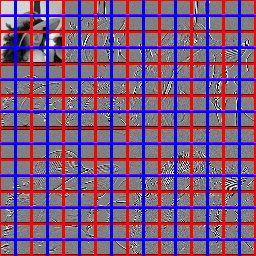
\includegraphics[width=4cm]{images/LaBouteWvltBlocks2.png}
\label{subfig:blocks2} }
\caption{Illustration of the block $\ell_1/\ell_2$-norm. \subref{subfig:noblock} sparsity of the image in an orthogonal wavelet decomposition (gray pixels corresponds to low coefficients); \subref{subfig:blocks1} a non-overlapping block structure; \subref{subfig:blocks2} splitting of a more complex overlapping block structure into two non-overlapping layers.}
\label{fig:blocks}
\end{figure}

In our numerical experiments where $\Hh \equiv \RNJ$, coefficients within each resolution level (from $1$ to $J_0$) and each subband are grouped according to all possible square spatial blocks of size $S \times S$; which can be decomposed into $S^2$ non-overlapping block structures.

	\subsubsection{Regularization $\mutv \normtv{W x}$}
	\label{sec:tv-reg}

The second regularization favors piecewise-smooth images, by inducing sparsity on its gradient \cite{ROF92}. The total variation semi-norm can be viewed as a specific instance of $\ell_1/\ell_2$-norm, $\normtv{y} = \normbktv{\gradient y}$, with
%
\begin{equation*}
 \gradient : \left\{ \begin{array}{rcc}
          \RNN & \longrightarrow &  \RG\\
          y    & \longmapsto & (V \ast y, H \ast y)
          \end{array} \right.%
\qobjq{and} \normbktv{\pa{v,h}} = \sum_{p \in \bbket{1,N}^2} \sqrt{{v_p}^2 + {h_p}^2} ~,
\end{equation*}
% 
where the image gradient is computed by finite differences through convolution with a vertical filter $V$ and a horizontal filter $H$, and $\Bb_{\mathrm{TV}}$ is clearly non-overlapping. For some special gradient filters, the modified TV semi-norm can be split into simple functions, see for instance \cite{CombettesPesquet08,Pustelnik11}. However, we consider more conventional filters
%
\begin{equation*}
V =\left( \begin{array}{cc}  -1 & 0 \\ 1 & 0 \end{array} \right)%
\qobjq{and}%
H =\left( \begin{array}{cc}  -1 & 1 \\ 0 & 0 \end{array} \right)
\end{equation*}
% 
centered in the upper-left corner. Introducing an auxiliary variable as ad\-vo\-ca\-ted in \eqref{eq:tilde-f}, the main difficulty remains to invert the operator $\pa{\Id + \ga \gradient \circ \adj{\gradient}}$, where $\adj{\gradient}$ is the adjoint of the gradient (i.e. $-$ the divergence operator). Under appropriate boundary conditions, this can be done in the Fourier domain in $O(N^2 \log(N))$ operations.

%%%%%%%%%%%%%%%%%%%%%%%%%%%%%%%%%%%%%%%%%%%%%%%%%%%%
\subsection{Resolution with Splitting Methods}

	\subsubsection{Tested Algorithms}

We now give the details of the different splitting strategies required to apply the three tested algorithms to \eqref{eq:vpb}.

\paragraph{Generalized Forward-Backward (\GFB)} The problem is rewritten under the form \eqref{eq:min} as
%
\begin{equation}\label{eq:vpb-GFB}
 \umin{\substack{x \in \Hh\\u \in \RG}} \half \norm{y - \Mr \Ks W x}^2 + \musp \sum_{i=1}^{S^2} \normbki{x} + \mutv \normbktv{u} + \iota_{C_{\gradient \circ W}}(x,u) ~,
\end{equation}
%
with $f(x) \equiv \half \norm{y - \Mr \Ks W x}^2$ and $n \equiv S^2 + 2$. The indicator function $\iota_{C_{\gradient \circ W}}$ is defined similarly as in \eqref{eq:tilde-f}. In \aref{algo:gfb}, we set equal weights $w_i \equiv 1/n$, a constant gradient step-size $\ga \equiv 1.8 \be$ and a constant relaxation parameter to $\la \equiv 1$.

\paragraph{Relaxed Douglas-Rachford (\DR)} Here the problem is split as
%
\begin{equation*}
 \umin{\substack{x \in \Hh\\u_1 \in \RNN\\u_2 \in \RG}} \half \norm{y - \Mr \, u_1}^2 + \iota_{C_{\Ks W}}(x,u_1) + \musp \sum_{i=1}^{S^2} \normbki{x} + \mutv \normbktv{u_2} + \iota_{C_{\gradient \circ W}}(x,u_2) ~,
\end{equation*}
% 
and solved with \aref{algo:gfb}, where $f \equiv 0$ and $n \equiv S^2 + 4$. As mentioned in \sref{sec:hybrid}, this corresponds to a relaxed version of the Douglas-Rachford algorithm. In our experiments, the best results were obtained for $\ga \equiv 1/n$.

\paragraph{Primal-Dual Chambolle-Pock (\ChPo)} A way to avoid operator inversions is to rewrite the original problem as
%
\begin{equation*}
  \umin{x \in \Hh} \, g (\La x)
\end{equation*}
% 
where
%
\begin{equation*}
 \La : \left\{ \begin{array}{ccc} \Hh & \longrightarrow & \RNN \times \pa{\Hh}^{S^2} \times \RG\\
     x & \longmapsto & \bpa{ \Mr \Ks W x, x, \dots, x, \gradient \circ W x} \end{array} \right.~,
\end{equation*}
% 
and
%
\begin{equation*}
g : \left\{ \begin{array}{rcl} \RNN \times \pa{\Hh}^{S^2} \times \RG & \longrightarrow & \R^+ \\
    \bpa{ u_1, x_1, \dots, x_{S^2}, g} & \longmapsto & \half \norm{y - u_1}^2 + \musp \sum_{i=1}^{S^2} \norm{x_i}_{1,2}^{\Bb_i} + \mutv \normbktv{g} \end{array} \right.~.
\end{equation*}
%
The operator $\La$ is a concatenation of linear operators and its adjoint is easy to compute, and $g$ is simple, being a separable sum of simple functions. Note that this is not the only splitting possible. For instance, one can write the problem on a product space as $\umin{\pa{x_i}_i \in \bHh} \iota_{\bSs}(\pa{x_i}_i) + \sum_i g_i(\La_i x_i)$, where $g_i$ is each of the functions in $g$ above, and $\La_i$ is each of the linear operators in $\La$.

To solve this, we here use the primal-dual relaxed Arrow-Hurwicz algorithm described in \cite{ChambollePock11}. According to the notations in that paper, we set the parameters $\sig \equiv 1$, $\tau \equiv \frac{0.9}{\sig(1+S^2+8)}$ and $\th \equiv 1$.

\paragraph{Block-Decomposition Hybrid Proximal Extragradient (\HPE)} We split the problem written in \eqref{eq:vpb-GFB} according to \eqref{eq:HPE}, and set equals weights $w_i \equiv 1/n$. According to \sref{sec:relations}, we set the parameter $\syg \equiv 0.9$.

\paragraph{Primal-Dual Combettes-Pesquet (\CoPe)} Finally, the problem takes its simplest form
%
\begin{equation}\label{eq:vpb-CoPe}
 \umin{x \in \Hh} \half \norm{y - \Mr \Ks W x}^2 + \musp \sum_{i=1}^{S^2} \normbki{x} + \mutv \normbktv{\gradient \circ W x}~.
\end{equation}
%
As long as $\mutv \equiv 0$ (no TV-regularization), this is exactly \eqref{eq:vpb-GFB}; we apply \aref{algo:CoPe} where $L_i \equiv \Id$ for all $i$ and $\ga \equiv 0.9/(1+S)$. However with TV-regularization, we avoid the introduction of the auxiliary variable $u$ with $L_{S^2+1} \equiv \gradient \circ W$ and $\ga \equiv 0.9/(1+\sqrt{S^2 + 8})$.

	\subsubsection{Results}

All experiments were performed on discrete images of width $N \equiv 256$, with values in the range $[0,1]$. The additive white Gaussian noise has standard-deviation $\sig_w \equiv 2.5 \cdot 10^{-2}$. The reconstruction operator $W$ uses separable bi-dimensional Daubechies wavelets with 2 vanishing moments. It is implemented such that each atom has norm $2^{-j}$, with $j \in \bbket{1,J_0}$ and where $J_0$ is the coarsest resolution level. Accordingly, we set the weights $\mu_\bk$ in the $\ell_1/\ell_2$-norm to $2^{-j}$ at the resolution level $j$ of the coefficients in block $\bk$. We use $J_0 \equiv 4$, resulting in a dictionary with redundancy $J = 3 J_0 +1 = 13$. All algorithms are implemented in \textsc{Matlab}\footnote{The codes for reproducing the experiments, as well as results on other images, are available at \url{http://www.ceremade.dauphine.fr/~raguet/gfb/}.}.

Results are presented in Figures \ref{fig:deconv}, \ref{fig:inpaint}, \ref{fig:composite} and \ref{fig:composite-tv}, %pp. \pageref{fig:deconv}-\pageref{fig:composite}. 
Only one image is shown here, but we obtained very similar results on other natural images (see \url{http://www.ceremade.dauphine.fr/~raguet/gfb/}). For each problem, the five algorithms were run $1000$ iterations (initialized at zero), while monitoring their objective functional values $F$ along iterations. $F_{\min}$ is fixed as the minimum value reached over the five algorithms (in our experiments, this was always that of \GFB), and evolution of the objectives compared to $F_{\min}$ is displayed for the first $100$ iterations. Because the computational complexity of an iteration may vary between algorithms, computation times for $100$ iterations (no parallel implementation) are given beside the curves. Below the objective decay graph, one can find from left to right the original image, the degraded image and the restored image after $100$ iterations of generalized forward-backward. Degraded and restored images quality are given in term of signal-to-noise ratio ($\ins{SNR}$).
 
\paragraph{Comparison to algorithms that do not use the (gradient) explicit step (\ChPo, \DR)} For the first three experiments, there is no total variation regularization. In the deblurring task (\cff{fig:deconv}), blocks of size $2 \times 2$ are used. \GFB is slightly faster than the others while the iteration cost of \ChPo is much higher for this problem. When increasing the block size (inpainting, \cff{fig:inpaint}, size $4 \times 4$) computation times tend to be similar but the decay of the objective  provided by \GFB is clearly faster than that of other algorithms. The advantage of using the gradient information becomes even more salient in the composite case (\ie $\Phi \equiv \Mr \Ks$): in \cff{fig:composite}, \DR performs hardly better than \ChPo. Indeed, in contrast to the previous cases (see \sref{sec:data-fid}), $f$ is not simple anymore and the introduction of the auxiliary variable decreases the efficiency of each iteration of \DR. This phenomenon is further illustrated in the last case, where the total variation is added, introducing another auxiliary variable.

\paragraph{Comparison to algorithms that use the (gradient) explicit step (\HPE, \CoPe)} In the first experiment where $n$ is small, the iterations of the suggested block-de\-com\-po\-si\-tion \HPE and \CoPe are almost as efficient as those of \GFB but take more time to compute, especially for \CoPe that needs two calls to $\nabla f$. Recall however that \HPE and \CoPe solve both the primal and dual problems. In the second setting, \HPE and \CoPe are hardly better than \DR. They perform better in the composite setting (\ie $\Phi \equiv \Mr \Ks$), but require more computational time than \GFB. In the last setting, iterations of \CoPe are still not as efficient as those of \GFB, despite the higher computational load due to the composition by the linear operator $\gradient \circ W$. %(see \aref{algo:CoPe}).

Finally, let us note that in the composite case, the $\ins{SNR}$ of the restored image is greater when using both regularizations rather than one or the other separately. Moreover, we observed that it yields restorations more robust to variations of the parameters $\musp$ and $\mutv$. Those arguments seem to be in favor of mixed regularizations.

%%%%%%%%%%%%%%%%%%%%%%%%%%%%%%%%%%%%%%%%%%%%%%%%%%%%
\floatstyle{boxed}
\restylefloat{figure}

\begin{figure}[p]
\bigcenter
\subfiguretopcaptrue
\subfigure[$\log(F - F_{\min})$ vs. iteration \#]{
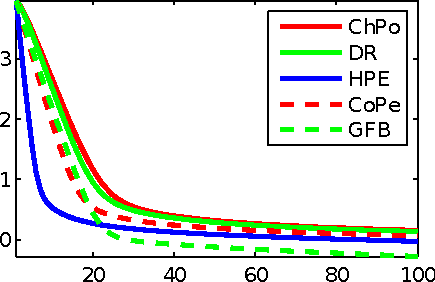
\includegraphics[width=.5\textwidth]{images/deblurring_l1l2_2_100_curves.pdf}
\label{subfig:deconv-curves}}
\subtable[computing time]{
\begin{tabular}{>{\Large}l>{\Large}l}
		   &		     \\
	$t_{\ChPo}$  &$= 153~\ins{s}$\\
	$t_{\DR}$  &$= 95~\ins{s}$\\
	$t_{\HPE}$  &$= 148~\ins{s}$\\
	$t_{\CoPe}$ &$= 235~\ins{s}$\\
	$t_{\GFB}$ &$= 73~\ins{s}$\\
\end{tabular}} \\
\subfiguretopcapfalse
\subfigure[LaBoute $y_0$]{
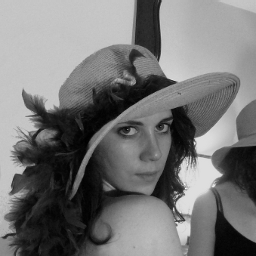
\includegraphics[width=.3\textwidth]{images/LaBoute.png}
\label{subfig:deconv-img} }
\subfigure[${y = \Ks y_0 + w}, \, 19.63~\ins{dB}$]{
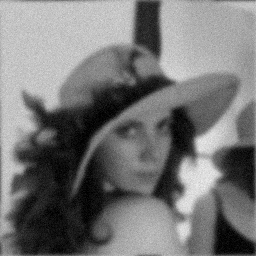
\includegraphics[width=.3\textwidth]{images/deblurring_l1l2_2_100_obs.png}
\label{subfig:deconv-obs} }
\subfigure[$\widehat{y}_0 = W\widehat{x}, \, 22.45~\ins{dB}$]{
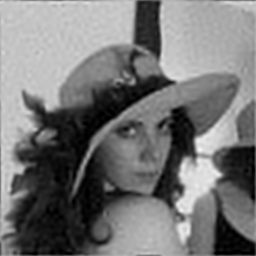
\includegraphics[width=.3\textwidth]{images/deblurring_l1l2_2_100_recov.png}
\label{subfig:deconv-recov} }
\caption{Deblurring: $\sig = 2$; $\musp = 1.3 \cdot 10^{-3}$; $S = 2$; $\mutv = 0$.}
\label{fig:deconv}
\end{figure}

\begin{figure}[p]
\bigcenter
\subfiguretopcaptrue
\subfigure[$\log(F - F_{\min})$ vs. iteration \#]{
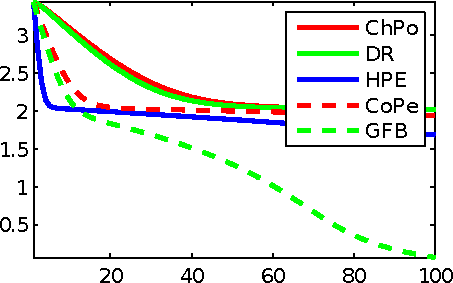
\includegraphics[width=.5\textwidth]{images/inpainting_l1l2_4_100_curves.pdf}
\label{subfig:inpaint-curves}}
\subtable[computing time]{
\begin{tabular}{>{\Large}l>{\Large}l}
		   &		     \\
	$t_{\ChPo}$  &$= 229~\ins{s}$\\
	$t_{\DR}$  &$= 219~\ins{s}$\\
	$t_{\HPE}$  &$= 352~\ins{s}$\\
	$t_{\CoPe}$ &$= 340~\ins{s}$\\
	$t_{\GFB}$ &$= 203~\ins{s}$\\
\end{tabular}} \\
\subfiguretopcapfalse
\subfigure[LaBoute $y_0$]{
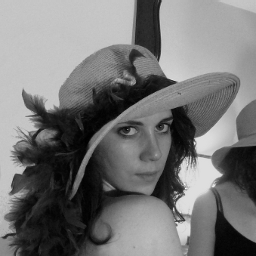
\includegraphics[width=.3\textwidth]{images/LaBoute.png}
\label{subfig:inpaint-img} }
\subfigure[$y = \Mr y_0 + w, \, 1.54~\ins{dB} $]{
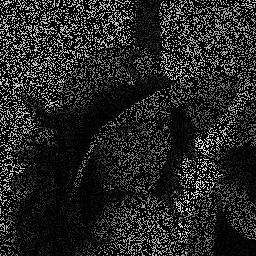
\includegraphics[width=.3\textwidth]{images/inpainting_l1l2_4_100_obs.png}
\label{subfig:inpaint-obs} }
\subfigure[$\widehat{y}_0 = W\widehat{x}, \, 21.66~\ins{dB}$]{
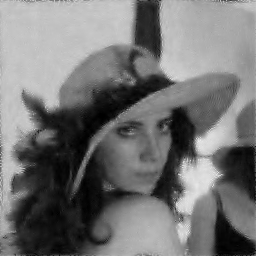
\includegraphics[width=.3\textwidth]{images/inpainting_l1l2_4_100_recov.png}
\label{subfig:inpaint-recov} }
\caption{Inpainting: $\rho = 0.7$; $\musp = 2.6 \cdot 10^{-3}$; $S = 4$; $\mutv = 0$.}
\label{fig:inpaint}
\end{figure}

\begin{figure}[p]
\bigcenter
\subfiguretopcaptrue
\subfigure[$\log(F - F_{\min})$ vs. iteration \#]{
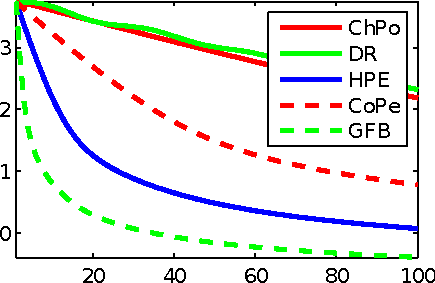
\includegraphics[width=.48\textwidth]{images/composite_l1l2_4_100_curves.pdf}
\label{subfig:composite-curves}}
\subtable[computing time]{
\begin{tabular}{>{\Large}l>{\Large}l}
		   &		     \\
	$t_{\ChPo}$  &$= 313~\ins{s}$\\
	$t_{\DR}$  &$= 256~\ins{s}$\\
	$t_{\HPE}$  &$= 342~\ins{s}$\\
	$t_{\CoPe}$ &$= 268~\ins{s}$\\
	$t_{\GFB}$ &$= 233~\ins{s}$\\
\end{tabular}} \\
\subfiguretopcapfalse
\subfigure[LaBoute $y_0$]{
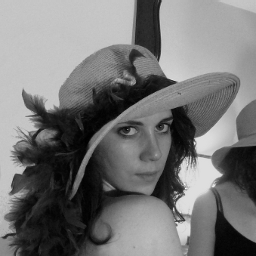
\includegraphics[width=.3\textwidth]{images/LaBoute.png}
\label{subfig:composite-img} }
\subfigure[$y = \Mr \Ks y_0 + w, \, 3.93~\ins{dB}$]{
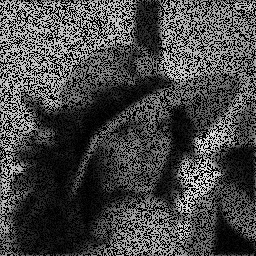
\includegraphics[width=.3\textwidth]{images/composite_l1l2_4_100_obs.png}
\label{subfig:composite-obs} }
\subfigure[$\widehat{y}_0 = W\widehat{x}, \, 20.77~\ins{dB}$]{

\includegraphics[width=.3\textwidth]{images/composite_l1l2_4_100_recov.png}
\label{subfig:composite-recov} }
\caption{Composite: $\sig = 2$; $\rho = 0.4$; $\musp = 1.0 \cdot 10^{-3}$; $S = 4$; $\mutv = 0$.}
\label{fig:composite}
\end{figure}

\begin{figure}[p]
\bigcenter
\subfiguretopcaptrue
\subfigure[$\log(F - F_{\min})$ vs. iteration \#]{
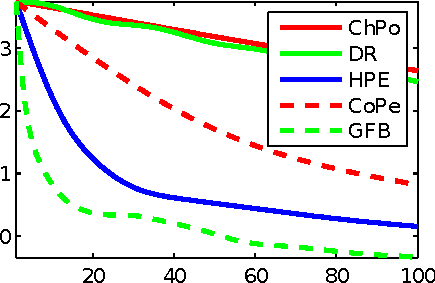
\includegraphics[width=.48\textwidth]{images/composite_l1l2_tv_4_100_curves.pdf}
\label{subfig:composite-tv-curves}}
\subtable[computing time]{
\begin{tabular}{>{\Large}l>{\Large}l}
		   &		     \\
	$t_{\ChPo}$  &$= 358~\ins{s}$\\
	$t_{\DR}$  &$= 294~\ins{s}$\\
	$t_{\HPE}$  &$= 409~\ins{s}$\\
	$t_{\CoPe}$ &$= 441~\ins{s}$\\
	$t_{\GFB}$ &$= 286~\ins{s}$\\
\end{tabular}} \\
\subfiguretopcapfalse
\subfigure[LaBoute $y_0$]{
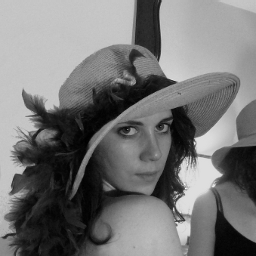
\includegraphics[width=.3\textwidth]{images/LaBoute.png}
\label{subfig:composite-tv-img} }
\subfigure[$y = \Mr \Ks y_0 + w, \, 3.93~\ins{dB}$]{
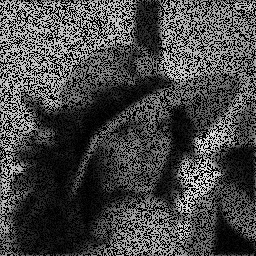
\includegraphics[width=.3\textwidth]{images/composite_l1l2_tv_4_100_obs.png}
\label{subfig:composite-tv-obs} }
\subfigure[$\widehat{y}_0 = W\widehat{x}, \, 22.48~\ins{dB}$]{
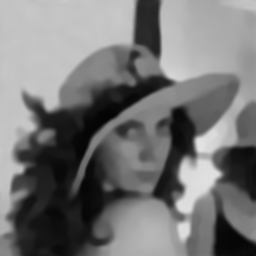
\includegraphics[width=.3\textwidth]{images/composite_l1l2_tv_4_100_recov.png}
\label{subfig:composite-tv-recov} }
\caption{Composite: $\sig = 2$; $\rho = 0.4$; $\musp = 5.0 \cdot 10^{-4}$; $S = 4$; $\mutv = 5.0 \cdot 10^{-3}$.}
\label{fig:composite-tv}
\end{figure}

\floatstyle{plain}
\restylefloat{figure}
%%%%%%%%%%%%%%%%%%%%%%%%%%%%%%%%%%%%%%%%%%%%%%%%%%%%

%%%%%%%%%%%%%%%%%%%%%%%%%%%%%%%%%%%%%%%%%%%%%%%%%%%%
%%%%%%%%%%%%%%%%%%%%%%%%%%%%%%%%%%%%%%%%%%%%%%%%%%%%
%%%%%%%%%%%%%%%%%%%%%%%%%%%%%%%%%%%%%%%%%%%%%%%%%%%%
\section{Convergence Proofs}
\label{sec:proofs}

This section is dedicated to the proof of convergence of the \GFB. We first recall some essential definitions and properties of monotone operator theory that are necessary to our exposition. The interested reader may refer to \cite{BauschkeCombettes11,Phelps93} for a comprehensive treatment. As we will deal with maximal monotone operator splitting, we then introduce specific notations on the product space $\Hh^n$. Finally, the proof itself is detailed in two steps. First, we derive an equivalent \textit{fixed point equation} satisfied by any solution of \eqref{eq:incl}. From this, we draw an algorithmic scheme (equivalent to \GFB) and establish its convergence properties and its robustness to summable errors.

%%%%%%%%%%%%%%%%%%%%%%%%%%%%%%%%%%%%%%%%%%%%%%%%%%%%
\subsection{Definitions and Properties}
\label{sec:defn-prop}

In the following, $A : \Hh \to 2^\Hh$ is a set-valued operator and $T : \dom T = \Hh \to \Hh$ is a full-domain (see below), single-valued operator. $\Id$ denotes the identity operator on $\Hh$.

\begin{definition}[Graph, inverse, domain, range and zeros]
\label{def:setvalued}
The \textit{graph} of $A$ is the set $\gra A \eqdef \setdef{(x,y) \in \Hh^2}{y \in Ax}$. The \textit{inverse} of $A$ is the operator whose graph is $\gra \inv{A} \eqdef \setdef{(x,y) \in \Hh^2}{(y,x) \in \gra A}$. The \textit{domain} of $A$ is $\dom A \eqdef \setdef{x \in \Hh}{Ax \neq \emptyset}$. The \textit{range} of $A$ is $\ran A \eqdef \setdef{y \in \Hh}{\existss x \in \Hh : y \in Ax}$, and its \textit{zeros} set is $\zer A \eqdef \setdef{x \in \Hh}{0 \in Ax} = \inv{A} \pa{0}$.
\end{definition}

\begin{definition}[Resolvent and reflection operators]
The \textit{resolvent} of $A$ is the operator $J_A \eqdef \inv{\bpa{\Id+A}}$. The \textit{reflection operator} associated to $J_A$ is the operator $R_A \eqdef 2 J_A - \Id$.
\end{definition}

\begin{definition}[Maximal monotone operator]
$A$ is \textit{monotone} if 
%
\[
	\foralls x,y \in \Hh, \quad \pa{ u \in Ax \sobjs{and} v \in Ay } \Rightarrow \dprod{u - v}{x - y} \geq 0~.
\]
%
It is moreover \textit{maximal monotone} if its graph is not strictly contained in the graph of any other monotone operator.
\end{definition}

\begin{definition}[Uniformly monotone operator]
$A$ is \textit{uniformly monotone} of modulus $\phy: [0,\pinfty[ \to [0,\pinfty]$ if $\phy$ is a non-decreasing function that vanishes only at 0, such that
%
\[
	\foralls x,y \in \Hh, \quad \pa{ u \in Ax \sobjs{and} v \in Ay } \Rightarrow  \dprod{u - v}{x - y} \geq \phy(\norm{x - y})~.
\]
%
\end{definition}
 
\begin{definition}[Non-expansive and $\al$-averaged operators]
$T$ is \textit{non-expansive} if 
%
\[ \foralls x,y \in \Hh, \qquad \norm{Tx - Ty} \leq \norm{x - y} ~. \]
%
For $\al \in ]0,1[$, $T$ is \textit{$\al$-averaged} if there exists $R$ non-expansive such that $T = (1-\al) \Id + \al R$. We denote $\Aa(\al)$ the class of $\al$-averaged operators on $\Hh$. In particular, $\Ademi$ is the class of \textit{firmly non-expansive} operators.
\end{definition}

\begin{definition}[cocoercive operator]
For $\be \in \, ]0,\pinfty[$, $T$ is $\be$-\textit{cocoercive} if $\be T \in \Ademi$.
\end{definition}

The following lemma gives some useful characterizations of firmly non-expansive operators.

\begin{lemma} The following statements are equivalent:
\begin{enumerate}[label={\rm (\roman{*})}, ref={\rm (\roman{*})}]
\item{\label{fne}} $T$ is firmly non-expansive;
\item{\label{refl}} $2T-\Id$ is non-expansive;
\item{\label{1-coco}} $\foralls x,y \in \Hh, \, \norm{Tx - Ty}^2 \leq \dprod{Tx - Ty}{x - y}$;
\item{\label{resolv}} $T$ is the resolvent of a maximal monotone operator $A$, \ie $T = J_{A}$.
\end{enumerate} 
\label{lem:fne}
\end{lemma}

\begin{proof}
\ref{fne} $\Leftrightarrow$ \ref{refl}, $T \in \Ademi \Leftrightarrow T = \frac{\Id + R}{2}$ for some $R$ non-expansive.
\ref{fne} $\Leftrightarrow$ \ref{1-coco}, see \cite{Zarantonello71}.
\ref{fne} $\Leftrightarrow$ \ref{resolv}, see \cite{Minty62}.
\end{proof}

Note that with \ref{1-coco}, one retrieves the characterization of the cocoercivity given in \sref{sec:algo}. It follows by the Cauchy-Schwarz inequality that $\be$-cocoercivity implies $1/\be$-Lipschitz continuity, but the converse is not true in general. It turns however to be the case for gradients of convex functionals. We summarize here some properties of the subdifferential.

\begin{lemma} Let $f : \Hh \to \R$ be a convex differentiable function, with $1/\be$-Lipschitz continuous gradient, $\be \in \, ]0,\pinfty[$, and let $g \in \Ga_0(\Hh)$. Then,
\begin{enumerate}[label={\rm (\roman{*})}, ref={\rm (\roman{*})}]
\item{\label{Baillon-Haddad}} $\be \nabla f \in \Ademi$, \ie is firmly non-expansive;
\item{\label{subd-max-mono}} $\partial g$ is maximal monotone;
\item{\label{Moreau}} The resolvent of $\partial g$ is the proximity operator of $g$, \ie $\prox_{g} = J_{\partial g}$.
\end{enumerate} 
\label{lem:subd}
\end{lemma}

\begin{proof}
\ref{Baillon-Haddad} This is Baillon-Haddad theorem \cite{BaillonHaddad77}.
\ref{subd-max-mono} See \cite{Rockafellar70}.
\ref{Moreau} See \cite{Moreau65}.
\end{proof}

%%%%%%%%%%%%%%%%%%%%%%%%%%%%%%%%%%%%%%%%%%%%%%%%%%%%
\subsection{Product Space}
\label{sec:prod-space}

Let $\pa{w_i}_{i \in \bbket{1,n}} \in {]0,1]}^n$ such that $\sum_{i=1}^n w_i = 1$. We consider $\bHh \eqdef \Hh^n$ endowed with the scalar product $\bdprod{\cdot}{\cdot}$, defined as
%
\begin{equation*}
  \foralls \bx = \pa{x_i}_i, \by = \pa{y_i}_i \in \bHh, \quad \bdprod{\bx}{\by} = \sum_{i=1}^n w_i \dprod{x_i}{y_i}
\end{equation*}
% 
and with the corresponding norm $\bnorm{\cdot}$. $\bSs \subset \bHh$ denotes the non-empty closed convex set defined by $\bSs \eqdef \setdef{ \bx = \pa{x_i}_i \in \bHh}{x_1 = x_2 = \cdots = x_n}$, whose orthogonal complement is the closed linear subspace $\bSs^\bot$. We denote by $\bId$ the identity operator on $\bHh$, and we define the canonical isometry 
%
\[ \bC: \Hh \to \bSs, x \mapsto (x,\ldots,x)~. \]
%
${ \iota_{\bSs} : \bHh \to ]\minfty,\pinfty] }$ and $N_{\bSs}: \bHh \to 2^{\bHh}$ are respectively the \textit{indicator function} and the \textit{normal cone} of $\bSs$, that is
%
\[
\iota_{\bSs}(\bx) \eqdef 
\begin{cases}
 0			& \sobjs{if}  \bx \in \bSs~, \\ 
 \pinfty		& \sobjs{otherwise}~,
 \end{cases} \quad \sobjs{and} \quad
N_{\bSs}(\bx) \eqdef 
\begin{cases}
 \bSs^\bot  & \sobjs{if}  \bx \in \bSs~, \\ 
 \emptyset   & \sobjs{otherwise}~.
 \end{cases}
\]
%
Since $\bSs$ is non-empty closed and convex, it is straightforward to see that $N_{\bSs}$ is maximal monotone.

We also introduce the following concatenated operators. Fix $B$ and the $A_i$'s in problem \eqref{eq:incl}. Given $\bga = \pa{\ga_i}_{i \in \bbket{1,n}} \in {]0,\pinfty[}^n$, we define
%
\[
	{\bgaA : \bHh \to 2^{\bHh}}, \bx = \pa{x_i}_i \mapsto \bigtimes_{i=1}^n \ga_i A_i(x_i)~,
\]
%
\ie its graph is
%
\begin{eqnarray*}
\gra \bgaA & \eqdef & \bigtimes_{i=1}^n \gra \ga_i A_i\\
	       & =      & \setdef{(\bx,\by) \in {\bHh}^2}{\bx = \pa{x_i}_i, \by = \pa{y_i}_i, \sobjs{and} \foralls i, \, y_i \in \ga_i A_i x_i}~,
\end{eqnarray*}
%
and $\bB : \bHh \to \bHh, \bx = \pa{x_i}_i \mapsto \pa{B x_i}_i$. Using the maximal monotonicity of the $A_i$'s and the $\be$-cocoercivity of $B$, it is an easy exercise to establish that $\bgaA$ is maximal monotone and $\bB$ is $\be$-cocoercive on $\bHh$.

%%%%%%%%%%%%%%%%%%%%%%%%%%%%%%%%%%%%%%%%%%%%%%%%%%%%
\subsection{Fixed Point Equation}
\label{sec:fix-point}

Now that we have all necessary material, let us characterize solutions of \eqref{eq:incl}.

\begin{proposition} Let $\pa{w_i}_{i \in \bbket{1,n}} \in {]0,1]}^n$. For any $\ga > 0$, $x \in \Hh$ is a solution of \eqref{eq:incl} if and only if there exists $\pa{z_i}_{i \in \bbket{1,n}} \in \Hh^n$ such that
%
\begin{equation}\label{eq:zi}
  \left\{ \begin{array}{L}
	\foralls i, \, z_i = \RgAi ( 2x - z_i - \ga B x ) - \ga B x ~, \\
	x = \textsum{i}{} w_i z_i ~.
\end{array}\right.
\end{equation}
%
\label{prop:fix-zi}
\end{proposition}

\ifx\siam\undefined \begin{proof} \else {\em Proof}. \fi
set $\ga > 0$, we have the equivalence
%
\begin{eqnarray*}
 0 \in B x + \sum_i A_i x & \Leftrightarrow & \existss \pa{z_i}_i \in \Hh^n :\, %
\left\{ \begin{array}{l}
	\foralls i, \, w_i \pa{x - z_i - \ga B x} \in \ga A_i x ~, \\
	x = \sum_i w_i z_i ~.
\end{array}\right.
\end{eqnarray*}
%
Now,
\begin{eqnarray*}
w_i \pa{x - z_i - \ga B x} \in \ga A_i x 
	& \Leftrightarrow & (2x - z_i - \ga B x) - x \in \frac{\ga}{w_i} A_i x \\
\intext{(by \lref{lem:fne}~\ref{resolv})} & \Leftrightarrow & \hphantom{2}x = \JgAi(2x-z_i-\ga B x) \\
	& \Leftrightarrow & 2x - (2x - z_i) = 2 \JgAi(2x - z_i - \ga B x) \\
	& 		  & \hphantom{2x - (2x - z_i) = } - (2x - z_i - \ga B x) - \ga B x \\
  	& \Leftrightarrow & \hphantom{2}z_i = \RgAi(2x - z_i - \ga B x) - \ga B x ~.
\ifx\siam\undefined \else \qquad\endproof \fi
\end{eqnarray*}
\ifx\siam\undefined \end{proof} \fi

From now on, to lighten the notation, we denote $\PS \eqdef J_{N_{\bSs}}$ and $\RS \eqdef R_{N_{\bSs}}$. Before formulating our fixed point equation, we need the following preparatory lemma.

\begin{lemma} For all $\bz = \pa{z_i}_i \in \bHh$, $\bb = \pa{b}_i \in \bSs$, and $\bga = \pa{\ga_i}_i \in {]0,\pinfty[}^n$,
\begin{enumerate}[label={\rm (\roman{*})}, ref={\rm (\roman{*})}]
\item{\label{proj-S}} $\PS$ is the \textit{orthogonal projector} on $\bSs$, and $\PS \bz = \bC\bpa{\sum_i w_i z_i}$;
\item{\label{refl-S}} $\RS \pa{ \bz - \bb } = \RS \bz - \bb$;
\item{\label{RgA}} $\RgA \bz = \bpa{\RgiAi(z_i)}_i$.
\end{enumerate}
\label{lem:JRSA}
\end{lemma}

\ifx\siam\undefined \begin{proof} \else {\em Proof}. \fi

\ref{proj-S}.~From \lref{lem:subd}~\ref{Moreau}, we have for $\bz \in \bHh$, 
%
\begin{equation*}
\PS(\bz) = {\argmin_{\by \in \bSs} \bnorm{\bz - \by}} \eqdef \proj_{\bSs}(\bz)~.
\end{equation*}
% 
Now, ${\argmin_{\by \in \bSs} \bnorm{\bz - \by}^2} = \bC\pa{\argmin_{y \in \Hh} \sum_i w_i \norm{z_i - y}^2}$, where the uni\-que minimizer of $\sum_i w_i \norm{z_i - y}^2$ is the barycenter of $\pa{z_i}_i$, \ie $\sum_i w_i z_i$.

\ref{refl-S}.~$\PS$ is obviously linear, and so is $\RS$. Since $\bb \in \bSs$, $\RS \bb = \bb$ and the result follows.

\ref{RgA}.~This is a consequence of the separability of $\bgaA$ in terms of the components of $\bz$ implying that $\JgA \bz = \pa{\JgiAi z_i}_i$. The result follows from the definition of $\RgA$.
\ifx\siam\undefined \end{proof} \else \endproof \fi

In the sequel, we denote the set of \textit{fixed points} of an operator $\bT : \bHh \to \bHh$ by $\fix \bT \eqdef \setdef{\bz \in \bHh}{\bT \bz = \bz}$.
\begin{proposition}
$\pa{z_i}_{i \in \bbket{1,n}} \in \Hh^n$ satisfies \eqref{eq:zi} if and only if  $\bz = \pa{z_i}_i$ is a fixed point of the following operator
%
\begin{equation}\label{eq:operator}
\begin{array}{rcl} \bHh & \longrightarrow & \bHh \\
	\bz & \longmapsto & \half \big[ \RgA  \RS + \bId \big]  \big[ \bId - \ga \bBJ \big](\bz) ~,
\end{array}
\end{equation}
%
with $\bga = \pa{\frac{\ga}{w_i}}_i$.
\label{prop:fix-z}
\end{proposition}

\ifx\siam\undefined \begin{proof} \else {\em Proof.} \fi
%
Using \lref{lem:JRSA} in \eqref{eq:zi}, we have $\bC(x) = \PS \bz$, $\bC(B x) = \bBJ(\bz)$ and $\RS - \ga \bBJ = \RS  [\bId - \ga \bBJ]$. Altogether, this yields,
%
\begin{eqnarray*}
 \bz \sobjs{satisfies} \eqref{eq:zi} & \Leftrightarrow & \hphantom{2}\bz = \RgA \RS \big[ \bId - \ga \bBJ \big] \bz - \ga \bBJ \bz  \\
  & \Leftrightarrow & 2 \bz = \RgA \RS \big[ \bId - \ga \bBJ \big] \bz + \big[ \bId - \ga \bBJ \big] \bz  \\
  & \Leftrightarrow & \hphantom{2}\bz = \half \big[ \RgA \RS + \bId \big] \big[ \bId - \ga \bBJ \big] \bz~.
\ifx\siam\undefined \else \qquad\endproof \fi
\end{eqnarray*}
\ifx\siam\undefined \end{proof} \fi

%%%%%%%%%%%%%%%%%%%%%%%%%%%%%%%%%%%%%%%%%%%%%%%%%%%%
\subsection{Properties of the Fixed Point Operator}
\label{sec:fix-pointop}
Expression \eqref{eq:operator} gives us the operator on which is based our \GFB scheme. We first study the properties of this operator that will play a crucial role in the convergence proof.

\begin{proposition}
For any $\bga \in {]0,\pinfty[}^n$, define
%
\begin{equation}\label{eq:Tb}
\Tb : \begin{array}{rcl} \bHh & \longrightarrow & \bHh \\
	\bz & \longmapsto & \half \left[ \RgA  \RS + \bId \right] \bz~.
\end{array}
\end{equation}
% 
Then, $\Tb$ is firmly non-expansive, \ie $\Tb \in \Ademi$.
\label{prop:Tb}
\end{proposition}

\begin{proof}
From \lref{lem:fne}~\ref{fne}$\Leftrightarrow$\ref{refl}, $\RgiAi$ and $\RS$ are non-expansive, and so is $\RgA$ in view of \lref{lem:JRSA}~\ref{RgA}. Finally, as a composition of non-expansive operators, $\RgA\RS$ is also non-expansive, and the proof is complete by definition of $\Ademi$.
\end{proof}

\begin{proposition}
For any $\ga \in ]0,2\be[$, define
%
\begin{equation}\label{eq:Tf}
\Tf : \begin{array}{rcl} \bHh & \longrightarrow & \bHh \\
	\bz & \longmapsto & \left[ \bId - \ga \bBJ \right] \bz ~.\end{array}
\end{equation}
%
Then, $\Tf \in \Aa \pa{ \frac{\ga}{2 \be} }$.
\label{prop:Tf}
\end{proposition}

\begin{proof}
By hypothesis, $\be B \in \Ademi$ and so is $\be\bB$. Then, from \lref{lem:fne}~\ref{1-coco}, we have for any $\bx, \by \in \bHh$
\begin{eqnarray}
 \bnorm{\be \bBJ \bx - \be \bBJ \by}^2 & \leq & \bdprod{\be \bBJ \bx - \be \bBJ \by}{\PS \bx - \PS \by} \nonumber\\
  & & = \bdprod{\be \PS \bBJ \bx - \be \PS \bBJ \by}{\bx - \by} \nonumber\\
  & & = \bdprod{\be \bBJ \bx - \be \bBJ \by}{\bx - \by} ~,\label{eq:mono-cont}
\end{eqnarray} 
where we derive the first equality from the fact that $\PS$ is self-adjoint (\lref{lem:JRSA}~\ref{proj-S}), and the second equality using that for all $\bx \in \bHh$, $\bB \PS \bx \in \bSs$. From \lref{lem:fne}~\ref{1-coco}$\Leftrightarrow$\ref{fne}, we establish that $\be \bBJ \in \Ademi$. We conclude using \cite[Lemma 2.3]{Combettes04}.
\end{proof}

\begin{proposition}
For all $\bga \in {]0,\pinfty[}^n$ and $\ga \in {]0,2\beta[}$, $\Tb\Tf \in \Aa(\al)$, with $\al = \max\bpa{\textfrac{2}{3},\textfrac{2}{1+2\be/\ga}}$.
\label{prop:TbTf}
\end{proposition}

\begin{proof}
As $\Tb$ and $\Tf$ are $\alpha$-averaged operators by \pref{prop:Tb} and \pref{prop:Tf}, it follows from \cite[Lemma 2.2 (iii)]{Combettes04} that their composition is also $\alpha$-averaged with the given value of $\alpha$. 
\end{proof}

\medskip

\noindent The following proposition defines a maximal monotone operator $\Apga$ which will be useful for characterizing the operator $\Tb$.
\begin{proposition}\label{Ap-fix-zer}
For all $\bga \in {]0,\pinfty[}^n$ there exists a maximal monotone operator $\Apga$ such that $\Tb = J_{\Apga}$. Moreover for all $\ga > 0$,
%
\begin{equation}\label{incApB}
\by = \Tb\Tf\bz \Leftrightarrow \bz - \by -\ga \bBJ\bz \in \Apga \by ~.
\end{equation}
% 
In particular,
\[
\fix \Tb \Tf = \zer \pa{\Apga + \ga \bBJ }~.
\]
\end{proposition}
\begin{proof}
The existence of $\Apga$ is ensured by \pref{prop:Tb} and \lref{lem:fne}~\ref{resolv}. Then for $\bz \in \bHh$,
\begin{eqnarray*}
 \by = \Tb \Tf \bz  & \Leftrightarrow & \by = \inv{\pa{\bId + \Apga}} \bpa{\bId - \ga \bBJ} \bz \\
                    & \Leftrightarrow &  \bz - \ga \bBJ\bz - \by \in \Apga\by ~.
\end{eqnarray*}
Taking $\by=\bz$ proves the second statement.
\end{proof}

\noindent Now, let us examine the properties of $\Apga$.

\begin{proposition}\label{Ap-incl}
For all $\bga \in \, {]0,\pinfty[}^{n}$ and $(\bu,\by) \in \bHh^2$
%
\begin{equation}\label{caracAp}
\bu \in \Apga \by \Leftrightarrow \pSs{\bu} - \pSp{\by} \in \bgaA \pa{ \pSs{\by} - \pSp{\bu} }~,
\end{equation}
%
where we denote for any $\bv \in \bHh$, $\pSs{\bv} \eqdef \projS\pa{\bv}$ and $\pSp{\bv} \eqdef \projP\pa{\bv}$.
\end{proposition}
\begin{proof}
First of all, by definition of $\Tb$ we have
%
\begin{eqnarray}
 \Tb & = & \half \left[ \pa{2\JgA - \bId} \pa{2\projS - \bId} + \bId \right] \nonumber\\
     & = & \half \left[ 2\JgA (\projS - \projP) - (\projS - \projP) + \projS + \projP \right] \nonumber\\
     & = & \JgA (\projS - \projP) + \projP~. \label{caracTb}
\end{eqnarray} 
%
Therefore,
%
\begin{eqnarray}
\bu \in \Apga \by & \Leftrightarrow & \Tb \pa{\bu + \by} = \by \nonumber\\
\intext{(by \eqref{caracTb})} & \Leftrightarrow & \JgA \pa{ \pSs{(\bu+\by)} - \pSp{(\bu+\by)} } = \by - \pSp{(\bu + \by)} = \pSs{\by} - \pSp{\bu} \nonumber\\
                  & \Leftrightarrow & \pSs{(\bu+\by)} - \pSp{(\bu+\by)} - \pSs{\by} + \pSp{\bu} \in \bgaA \pa{ \pSs{\by} - \pSp{\bu} } \nonumber\\
                  & \Leftrightarrow & \pSs{\bu} - \pSp{\by} \in \bgaA \pa{ \pSs{\by} - \pSp{\bu} }~. \nonumber
\end{eqnarray}
%
\end{proof}

%%%%%%%%%%%%%%%%%%%%%%%%%%%%%%%%%%%%%%%%%%%%%%%%%%%%
\subsection{Convergence}
\label{sec:convergence}
We are now ready to state the main convergence result of our relaxed and inexact \GFB splitting algorithm \eqref{eq:gfb-err-algo} to solve \eqref{eq:incl}.
\begin{theorem}
Let $\ga \in ]0,2\be[$, and set $\bga = \pa{\frac{\ga}{w_i}}_i \in {]0,\pinfty[}^n$, \\
let $\pa{\la_k}_{k \in \N}$ be a sequence in $\left]0,\min \bpa{\textfrac{3}{2},\textfrac{1}{2}+\textfrac{\be}{\ga}}\right[$,\\
set $\bz_0 \in \bHh$, and for every $k \in \N$, set
%
\begin{equation}\label{eq:gfb-err}
\bz_{k+1} = \bz_k + \la_k \bpa{\Tb \bpa{ \Tf \bz_k + \bEps_{2,k} } + \bEps_{1,k} - \bz_k}
\end{equation}
% 
where $\Tb$ (resp. $\Tf$) is defined in \eqref{eq:Tb} (resp. in \eqref{eq:Tf}),
and $\bEps_{1,k}, \bEps_{2,k} \in \bHh$. If
%
\begin{enumerate}[label={\rm (\roman{*})}, ref={\rm (\roman{*})}]
	\item{\label{h:non-empty}} $\zer\bpa{B+\sum_i A_i} \neq \emptyset$;
	\item{\label{h:lim-la}} $0 < \inf_{k \in \N} \la_k \leq \sup_{k \in \N} \la_k < \min \bpa{\textfrac{3}{2},\textfrac{1}{2}+\textfrac{\be}{\ga}}$;
	\item{\label{h:sum-err}} $\sum_{k=0}^{\pinfty} \bnorm{\bEps_{1,k}} < \pinfty$ and $\sum_{k=0}^{\pinfty} \bnorm{\bEps_{2,k}} < \pinfty$.
\end{enumerate} 
%
are satisfied, then
\begin{enumerate}[label={\rm (\alph{*})}, ref={\rm (\alph{*})}]
	\item{\label{claim:Tz}} $\bpa{\Tb \Tf \bz_k - \bz_k}_{k \in \N}$ converges strongly to $0$;
	\item{\label{claim:z}} $\pa{\bz_k}_{k \in \N}$ converges weakly to a point $\bz \in \fix \Tb \Tf$;
	\item{\label{claim:x}} $\bpa{x_k \eqdef \sum_i w_i\bz_{i,k}}_{k \in \N}$ converges weakly to $x \eqdef \sum_i w_i \bz_i \in \zer{\bpa{B+\sum_i A_i}}$.\\
		\newline
\item{\label{claim:strong}} Moreover, if $\foralls k \in \N, \, \la_k \leq 1$, $\pa{x_k}_{k \in \N}$ converges strongly in each of the following cases: 
\begin{enumerate}[label={\rm (\arabic{*})}, ref={\rm (\arabic{*})}]
\item{\label{claim:strongB}} $B$ is uniformly monotone.
\item{\label{claim:strongA}} $\bigtimes_{i=1}^n w_i^{-1} A_i$ is uniformly monotone. For instance, this is true if $\forall i \in \bbket{1,n}$, $A_i$ is uniformly monotone with the same modulus $\phy$ being also subadditive or convex.
\end{enumerate} 
\end{enumerate}
\label{thm:gfb}
\end{theorem}

\begin{proof}
\noindent\ref{claim:Tz}.
Denoting $\bT \eqdef \Tb \Tf$, we have for all $k \in \N$,
%
\begin{equation}\label{eq:T-Eps}
  \bz_{k+1} = \bz_k + \la_k \bpa{ \bT \bz_k + \bEps_{k} - \bz_k } ~,
\end{equation}
% 
with $\bEps_{k} \eqdef \Tb \bpa{ \Tf \bz_k + \bEps_{2,k} } - \Tb \bpa{ \Tf \bz_k } + \bEps_{1,k}$. \pref{prop:Tb} shows that $\Tb \in \Ademi$ is in particular non-expansive, so that $\bnorm{\bEps_k} \leq \bnorm{\bEps_{2,k}} + \bnorm{\bEps_{1,k}}$, and we deduce from \ref{h:sum-err} that $\sum_{k=0}^{\pinfty} \bnorm{\bEps_{k}} < \pinfty$. Moreover, by \pref{prop:TbTf}, $\bT \in \Aa(\al)$ with $\al = \max\bpa{\textfrac{2}{3},\textfrac{2}{1+2\be/\ga}}$. In particular, $\bT$ is non-expansive and thus $\fix \bT$ is closed and convex. Now, for $k \in \N$, set $\bT_k \eqdef \bId + \la_k \pa{\bT - \bId}$, the iterations \eqref{eq:T-Eps} can be rewritten
%
\begin{equation}\label{eq:Tt-Eps}
  \bz_{k+1} = \bT_k \bz_k + \la_k \bEps_{k} ~.
\end{equation}
% 
Since \ref{h:lim-la} provides for all $k \in \N$, $\al_k \eqdef \lambda_k \al < 1$, \cite[Lemma 2.2 (i)]{Combettes04} shows that $\bT_k \in \Aa(\al_k)$, and \eqref{eq:Tt-Eps} is thus a particular instance of \cite[Algorithm 4.1]{Combettes04}. Also, it is clear that for all $k \in \N$, $\fix \bT_k = \fix \bT$. Thus with \pref{prop:fix-zi} and \pref{prop:fix-z}, \ref{h:non-empty} provides $\bigcap_{k \in \N} \fix \bT_k = \fix \bT \neq \emptyset$. According to \ref{h:lim-la}, $\inf_{k \in \N} \la_k > 0$ and $\sup_{k \in \N} \al_k < 1$, so we deduce from \cite[Theorem~3.1 and Remark~3.4]{Combettes04} that
%
\begin{equation}\label{eq:assymp-reg}
\sum_{k \in \N} \bnormb{\bT_k \bz_k - \bz_k}^2 < \pinfty.
\end{equation}
% 
and that $\pa{\bz_k}_{k \in \N}$ is \textit{quasi-Fej\'er monotone} with respect to $\fix \bT$. By definition of $\bT_k$, \eqref{eq:assymp-reg} gives ${\sum_{k \in \N} {\la_k}^2 \bnormb{\bT \bz_k - \bz_k}^2 < \pinfty}$, which in turn implies $\bT \bz_k - \bz_k \cv 0$ since $\inf_{k \in \N} \la_k > 0$.\\

\noindent\ref{claim:z}.
$\bT$ being non-expansive, it follows from the demiclosed principle \cite{Browder67}\cite[Corollary~4.18]{BauschkeCombettes11} that any weak cluster point of $\pa{\bz_k}_{k\in\N}$ belongs to $\fix \bT$, so that \cite[Theorem~5.5]{BauschkeCombettes11} provides weak convergence towards $\bz \in \fix \bT$.\\

\noindent\ref{claim:x}.
For any $y \in \Hh$, $\dprod{y}{x_k-x} = \dprod{y}{\sum_i w_i(\bz_{i,k}-\bz_i)} = \sum_i w_i \dprod{y}{\bz_{i,k} - \bz_i} = \bdprod{\bC(y)}{\bz_k - \bz}$. So, \ref{claim:z} provides weak convergence of $\pa{x_k}_{k \in \N}$ towards $x$, which is a zero of $B + \sum_i A_i$ by \pref{prop:fix-zi}.\\


\noindent\ref{claim:strong}.
If moreover $\foralls k \in \N, \, \la_k \leq 1$, in view of \pref{prop:Tb} and \pref{prop:Tf}, \eqref{eq:gfb-err} is immediately a particular instance of \cite[Algorithm 4.1]{Combettes04}. In particular, \cite[Theorem~3.1 and Remark~3.4]{Combettes04} provides
%
\begin{equation}\label{eq:Id-Tfz}
	\sum_{k \in \N} \normb{(\bId - \Tf) \bz_k - (\bId - \Tf) \bz}^2 =%
	\sum_{k \in \N} \ga^2 \normb{\bBJ \bz_k - \bBJ \bz}^2 < \pinfty~,
\end{equation} 
%

\ref{claim:strong}\ref{claim:strongB}.
Now, if $B$ is uniformly monotone, then we have for all $k \in \N$,
%
\begin{eqnarray*}
\bdprod{\bBJ \bz_k - \bBJ \bz}{\bz_k - \bz} 
	& = & \textsum{i}{} w_i \dprod{B \bpa{ \textsum{i}{} w_i z_{i,k} } - B \bpa{ \textsum{i}{} w_i z_i}}{z_{i,k} - z_i} \\
	& = & \dprod{B \bpa{ \textsum{i}{} w_i z_{i,k} } - B \bpa{ \textsum{i}{} w_i z_i}}{\textsum{i}{} w_i (z_{i,k} - z_i)} \\
	& \geq & \phy \bpa{ \norm{x_k - x} }~.
\end{eqnarray*}
%
From \ref{claim:z} and \eqref{eq:Id-Tfz}, we deduce that the right-hand side of the last inequality converges to 0. In view of the properties of $\phy$, we obtain strong convergence of $\pa{x_k}_{k\in\N}$ towards $x$.

\ref{claim:strong}\ref{claim:strongA}.
Let $\bu = -\ga\bBJ\bz$ and $\foralls k \in \NN$,
\begin{eqnarray*}
\by_k = \Tb \Tf \bz_k \quad \text{and} \quad \bu_k = (\bz_k - \by_k) - \ga \bBJ\bz_k ~.
\end{eqnarray*}
We then have
\[
\normb{\bu_k - \bu} \leq \bnorm{\by_k-\bz_k} + \ga \normb{\bBJ \bz_k - \bBJ \bz} ~.
\]
It then follows from \ref{claim:Tz} and \eqref{eq:Id-Tfz} that $\bu_k$ converges strongly to $\bu$. On the other hand, by \pref{Ap-fix-zer}, we have
\[
\bu \in \Apga\bz \quad \text{and} \quad \bu_k \in \Apga\by_k ~.
\]
Therefore, applying \pref{Ap-incl} to the pairs $(\bz,\bu)$ and $(\by_k,\bu_k)$, and using the fact that $\bigtimes_{i=1}^n w_i^{-1} A_i$ is uniformly monotone, we obtain
\begin{eqnarray*}
\dprod{(\pSs{\bu}-\pSp{\bz})-(\pSs{\bu}_k-\pSp{\by}_k)}{(\pSs{\bz}-\pSp{\bu})-(\pSs{\by}_k-\pSp{\bu}_k)} \geq \phy\pa{\normb{(\pSs{\bz}-\pSp{\bu})-(\pSs{\by}_k-\pSp{\bu}_k)}}.
\end{eqnarray*}
for some non-decreasing function $\phy: [0,\pinfty[ \to [0,\pinfty]$ that vanishes only at $0$. We then have
\begin{eqnarray*}
\dprod{(\pSs{\bu}-\pSp{\bz})-(\pSs{\bu}_k-\pSp{\by}_k)}{(\pSs{\bz}-\pSp{\bu})-(\pSs{\by}_k-\pSp{\bu}_k)} &=&
\dprod{(\pSs{\bu}-\pSs{\bu}_k)-(\pSp{\bz}-\pSp{\by}_k)}{(\pSs{\bz}-\pSs{\by}_k)-(\pSp{\bu}-\pSp{\bu}_k)} \\
&=& \dprod{\pSs{\bu}-\pSs{\bu}_k}{\pSs{\bz}-\pSs{\by}_k}+\dprod{\pSp{\bz}-\pSp{\by}_k}{\pSp{\bu}-\pSp{\bu}_k} \\
&=& \dprod{\bu-\bu_k}{\bz-\by_k} ~.
\end{eqnarray*}
Moreover,
\begin{eqnarray*}
\phy\pa{\normb{(\pSs{\bz}-\pSp{\bu})-(\pSs{\by}_k-\pSp{\bu}_k)}} &=& \phy\pa{\normb{(\pSs{\bz}-\pSs{\by}_k)-(\pSp{\bu}-\pSp{\bu}_k)}} \\
&=& \phy\pa{\sqrt{\normb{\pSs{\bz}-\pSs{\by}_k}^2+\normb{\pSp{\bu}-\pSp{\bu}_k}^2}}\\
&\geq& \phy\pa{\normb{\pSs{\bz}-\pSs{\by}_k}}
\end{eqnarray*}
since $\phy \circ \sqrt{\cdot}: [0,\pinfty[ \to [0,\pinfty]$ is non-decreasing. Altogether, we arrive at
\[
\phy\pa{\normb{\pSs{\bz}-\pSs{\by}_k}} \leq \dprod{\bu-\bu_k}{\bz-\by_k} ~.
\]
By \ref{claim:Tz} and \ref{claim:z}, $\by_k$ converges weakly to $\bz$ and we have shown that $\bu_k$ converges strongly to $\bu$. This proves that $\dprod{\bu-\bu_k}{\bz-\by_k} \to 0$ and therefore $\pSs{\by}_k$ converges strongly to $\pSs{\bz}=x$ in view of the properties of $\phy$. The latter in conjunction with \ref{claim:Tz} implies that $\pSs{\bz}_k=x_k$ converges strongly to $x$.

It remains to show the special cases implying uniform monotonicity in \ref{claim:strong}\ref{claim:strongA}. Indeed, if $\foralls i \in \bbket{1,n}$, $A_i$ is uniformly monotone with the same modulus $\phy$ which is also convex, then for $(\bx,\bu) \in \gra \bgaA$ and $(\by,\bv) \in \gra \bgaA$,
\begin{eqnarray*}
\bdprod{\bu-\bv}{\bx-\by} =\sum_i w_i \dprod{u_i-v_i}{x_i-y_i} 
&\geq& \sum_i w_i \ga_i \phy\pa{\norm{x_i-y_i}} \\
(\text{\small $0 < \inf_i \ga_i < \infty$}) &\geq& \inf_i \ga_i ~ \sum_i w_i \phy\pa{\norm{x_i-y_i}} \\
(\text{\small $\phy$ is convex}) &\geq& \inf_i \ga_i ~ \phy\pa{\sum_i w_i \norm{x_i-y_i}} \\
(\text{\small $\phy$ is non-decreasing}) &\geq& \inf_i \ga_i ~ \phy\pa{\inf_i w_i \sqrt{\sum_i \norm{x_i-y_i}^2}} \\
(\text{\small $\phy$ is non-decreasing and $w_i \in ]0,1]$}) &\geq& \inf_i \ga_i ~ \phy\pa{\inf_i w_i \sqrt{\sum_i w_i \norm{x_i-y_i}^2}} \\
&=& \inf_i \ga_i ~ \phy\pa{\inf_i w_i ~ \bnorm{\bx-\by}} ~.
\end{eqnarray*}
The proof for the case where $\phy$ is subadditive follows the same lines using subadditivity instead of convexity in the inequalities, and replacing $\inf_i \ga_i$ by $\ga$ (since by definition $\ga_iw_i=\ga$) and $\inf_i w_i$ by $1$.
\end{proof}
{~}\\

\begin{remark}
\label{rem:ext-la}
For statements \ref{claim:Tz}-\ref{claim:x}, assumptions \ref{h:lim-la} can be weakened. More precisely, \ref{h:lim-la} can be replaced by $\sum_{k \in \N} \la_k(1-\al\la_k) = \pinfty$ where $\alpha=\max\bpa{\textfrac{2}{3},\textfrac{2}{1+2\be/\ga}}$, and \ref{h:sum-err} by $\sum_{t\in\N} \lambda_k (\bnorm{\bEps_{1,k}} + \bnorm{\bEps_{2,k}}) < \pinfty$. The proof would follow the same lines as \cite[Lemma~5.1]{Combettes04}. 
\end{remark}

\begin{remark}[Strong Convergence]
\label{rem:strong}
We have proved strong convergence of the sequence $\pa{x_k}_{k \in \N}$, but we did not elaborate on strong convergence of $\pa{z_k}_{k \in \N}$. It turns out that the sequence $\pa{\bz_k}_{k \in \N}$ is indeed quasi-Fej\'er monotone with respect to $\fix \bT$. Thus, if $\inte \pa{\fix \bT} \neq \emptyset$, \cite[Lemma~2.8(iv)]{Combettes04} provides strong convergence of $\pa{\bz_k}_{k \in \N}$, and therefore of $\pa{x_k}_{k \in \N}$. An alternative sufficient condition is that $\Apga$ is demiregular; see \cite[Definition~2.3]{Attouch10} and also \cite[Condition~3.2]{CombettesWajs05} in the case of convex optimization. Demiregularity occurs for instance if the operator has a boundedly relatively compact domain (the intersection of its closure with any closed ball is compact); see \cite[Proposition 2.4]{Attouch10}. However, this condition is rather abstract and it is not easy to translate it in terms of the properties of the individual $A_i$'s when $n > 1$.
%The sufficient condition of strong convergence can be weakened, and other ones can be stated as well. Indeed, our \GFB has a structure that bears similarities with the classical forward-backward, since it consists of an explicit forward step, followed by an implicit step where the resolvents are computed in parallel. In fact, it turns out that the backward step involves a firmly non-expansive operator (see \sref{sec:convergence}), and therefore statements of \cite[Theorem~3.4(iv) and Proposition 3.6]{CombettesWajs05} with constant step-size $\ga$ can be transposed with some care to our algorithm.
\end{remark} 

\begin{remark}[Non-stationary GFB]
\label{rem:nonstat}
Convergence of the non-stationary version of our inexact \GFB splitting algorithm, i.e. for a varying sequence $\pa{\ga_k}_{k \in \N}$, can also be established. More precisely, it can be shown that the statements of \tref{thm:gfb} hold under the additional assumption that $0 < \infga \leq \ga_k \leq \supga < 2\be$ and $\pa{\ga_k-\ga}_{k \in \N}$ is absolutely summable where $\ga \in [\infga,\supga]$. The key idea underlying the proof consists in viewing the non-stationary method as a perturbed version of the stationary method with an additional error term (beside those previously considered in the implicit and explicit steps), and to ensure that this error is also summable; see the initial work of \cite{Lemaire96a,Lemaire96b} in this direction. This absolute summability assumption on $\pa{\ga_k-\ga}_{k \in \N}$ can be dropped for $n \equiv 1$, in which case we recover the forward-backward algorithm.
\end{remark} 

Finally, let us explicit the relationship between \tref{thm:gfb} and the claims of \sref{sec:algo}.

\ifx\siam\undefined \begin{proof}[Proof of \tref{thm:gfb-algo}]
\else {\em Proof of \tref{thm:gfb-algo}}. \fi
%
It is straightforward to see that the vector whose coordinates are the sequences $\pa{z_{i,k}}_{k \in \N}$ defined in \eqref{eq:gfb-err-algo} follows iterations \eqref{eq:gfb-err}, with $\bEps_{1,k} = \pa{\Eps_{1,k,i}}_i$ and $\bEps_{2,k} = \bC \pa{ - \ga \Eps_{2,k} }$, which are of course summable under the required assumptions. Applying \tref{thm:gfb}, the claimed convergence properties follow.
\ifx\siam\undefined \end{proof} \else \endproof \fi


\ifx\siam\undefined \begin{proof}[Proof of \cref{cor:min}]
\else {\em Proof of \cref{cor:min}}. \fi
Under \ref{H:argmin}-\ref{H:sri}, \cite[Theorem~16.2 and Theorem~16.37(i)]{BauschkeCombettes11} provides that $\argmin(f + \sum_i g_i) = \zer{\pa{\nabla f + \sum_i \partial g_i}} \neq \emptyset$. Furthermore, in \lref{lem:subd}\ref{Baillon-Haddad} provides that $\nabla f$ is $\be$-cocoercive and \lref{lem:subd}\ref{Moreau} shows that $\JgAi$ corresponds to $\prox_{\!\frac{\ga}{w_i}\!g_i}$. Hence, weak convergence of $\pa{x_k}_{k \in \N}$ towards a minimizer of \eqref{eq:min} follows from \tref{thm:gfb}~\ref{claim:x}. The proof of strong convergence is a consequence of \tref{thm:gfb}~\ref{claim:strong} together with the fact that uniform convexity of a function in $\Ga_0(\Hh)$ implies uniform monotonicity of its subdifferential \cite{BauschkeCombettes11}.
%
\ifx\siam\undefined \end{proof} \else \endproof \fi

%%%%%%%%%%%%%%%%%%%%%%%%%%%%%%%%%%%%%%%%%%%%%%%%%%%%
%%%%%%%%%%%%%%%%%%%%%%%%%%%%%%%%%%%%%%%%%%%%%%%%%%%%
%%%%%%%%%%%%%%%%%%%%%%%%%%%%%%%%%%%%%%%%%%%%%%%%%%%%
\section{Conclusion}

We have introduced in this paper a novel splitting method for finding a zero of a sum of an arbitrary number of maximal monotone operator. It takes advantage of either the cocoercivity, or the possibility to compute the resolvent of each operator separately. We provided theoretical guarantees on the convergence of the algorithm and its robustness to summable errors. We emphasized the corresponding novel primal proximal splitting method for minimizing convex functionals that are the sum of a smooth term and several simple functions. It generalizes some existing schemes and enlarges the class of problems that can be solved efficiently with proximal splitting methods. Numerical experiments on convex optimization for inverse problems show evidence of the advantages of our approach for large-scale imaging problems.
